\documentclass[UTF8]{ctexart}
\usepackage{abstract}
\usepackage{lettrine}
\usepackage{multicol}
\usepackage{cite}
\usepackage{mathtools}
\usepackage{graphicx}
\usepackage{subfigure}
\usepackage{caption}
\usepackage{booktabs}
\usepackage{multirow}
\usepackage{diagbox}
\usepackage{makecell}
\usepackage{placeins}
\usepackage{float}
\usepackage{geometry}
\usepackage{amssymb}
\usepackage{xcolor}
\usepackage{soul}
\usepackage{rotating}
\usepackage{hyperref}
\newtheorem{1}{例}
\newtheorem{2}{解}
\newtheorem{3}{练习}
\newtheorem{4}{答案}
%\pagecolor[rgb]{0.1, 0.1, 0.1}
%\pagecolor[rgb]{0.4, 0.4, 0.4}
%\pagecolor{black} 
%\definecolor{Firebrick4}{RGB}{255, 255, 255}
%\definecolor{shadecolor}{rgb}{0.92,0.92,0.92}
%\textcolor[rgb]{1,0,0}{text}
%\textcolor{red/blue/green/black/white/cyan/magenta/yellow}{text}
%没有缩进           \noindent
%粗体,放大         {\bf\large 12}:12
%另段:           空行
%空行另段:      \\+空行
%文内插入公式如  $F_s=m_sa$
%单行插入公式   \begin{equation}
%               \end{equation}
%              \begin{displaymath}
%             \end{displaymath}
%乘号         \times
%分号         \dfrac{a}{b}
%绝对值      \left|a \right|
%根号        \sqrt{a}
%            \sqrt[3]{0}
%大于等于     \geq 0
%小于等于     \leq 0
%不等于        \ne 0   (b\ne 0)
%k属于R      a> 0,($k \in R $)
%集合   N:非负整数集合或自然数集合du{0,1,2,3,…}
%       Z:整数集合zhi{…,-1,0,1,…}
%       Q:有理数集合
%       R:实数集合(包括有理数和无理数)

%       R+:正实数集合
%       R-:负实数集合
%       C:复数集合
%       ∅ :空集(不含有任何元素的集合)
%       N*或N+:正整数集合{1,2,3,…}
%       Q+:正有理数集合
%       Q-:负有理数集合
%       省略号就用\cdots了
%      求和要加\displaystyle
%空格    \qquad 
\begin{document}
	%\markright{页眉}
%封面
\title{系数阵笔记1.8}
\author{浩于长空}
%\date{}
\maketitle
$$\text { Show that if } a, b, c,\geq 0,(a b+b c+c a)\left(\dfrac{1}{(a+b)^{2}}+\dfrac{1}{(b+c)^{2}}+\dfrac{1}{(c+a)^{2}}\right) \geq \dfrac{9}{4}
$$
\begin{flushright}
	\text { (Crux Problem No.1940 \& Iran TST,1996) }
\end{flushright}
\begin{displaymath}
\end{displaymath}
%摘要
\begin{abstract}
	有关三元齐次不等式的小讲堂的笔记,不会对高考或竞赛很有用……大家看心情看
	这里很多内容会很抽象很玄学,而且这个技术更像心法,未必能把自己的思考完全传达出来,能不能听懂全靠缘分,能保证的是Iran96这种简单的不等式以后遇到轻松解决。
\end{abstract}

\newpage

$$ (\displaystyle \sum ab)(\displaystyle \sum \dfrac{1}{(a+b)^{2}})\geq \dfrac{9}{4}$$
$$\Leftrightarrow 
4(\displaystyle \sum xy)(\displaystyle \sum (b+c)^{2}(c+a)^{2})\geq 9\prod (x+y)^{2}$$
$$\Leftrightarrow 
4\left[
\begin{smallmatrix}
	0& &1& &0\\
	&1& &1&\\
	& &0& &\\
\end{smallmatrix}
\right]
\displaystyle \sum \left[
\begin{smallmatrix}
	0& &0& &1& &0& &0\\
	&0& &2& &2& &0&\\
	& &1& &4& &1& &\\
	& & &2& &2& & &\\
	& & & &1& & & &\\
\end{smallmatrix}
\right]\geq 9\prod 
\left[
\begin{smallmatrix}
	1& &2& &1\\
	&0& &0&\\
	& &0& &\\
\end{smallmatrix}
\right]
$$
$$\Leftrightarrow 
4\left[
\begin{smallmatrix}
	0& &1& &0\\
	&1& &1&\\
	& &0& &\\
\end{smallmatrix}
\right]
\left[
\begin{smallmatrix}
	1& &2& &3& &2& &1\\
	&2& &8& &8& &2&\\
	& &3& &8& &3& &\\
	& & &2& &2& & &\\
	& & & &1& & & &\\
\end{smallmatrix}
\right]\geq 9
\left[
\begin{smallmatrix}
	0& &0& &1& &2& &1& &0& &0\\
	&0& &2& &6& &6& &2& &0&\\
	& &1& &6& &10& &6& &1& &\\
	& & &2& &6& &6& &2& & &\\
	& & & &1& &2& &1& & & &\\
	& & & & &0& &0& & & & &\\
	& & & & & &0& & & & & &\\
\end{smallmatrix}
\right]$$
$$\Leftrightarrow 
4\left[
\begin{smallmatrix}
	0& &1& &2& &3& &2& &1& &0\\
	&1& &5& &13& &13& &5& &1&\\
	& &2& &13& &24& &13& &2& &\\
	& & &3& &13& &13& &2& & &\\
	& & & &2& &5& &2& & & &\\
	& & & & &1& &1& & & & &\\
	& & & & & &0& & & & & &\\
\end{smallmatrix}
\right]\geq 9
\left[
\begin{smallmatrix}
	0& &0& &1& &2& &1& &0& &0\\
	&0& &2& &6& &6& &2& &0&\\
	& &1& &6& &10& &6& &1& &\\
	& & &2& &6& &6& &2& & &\\
	& & & &1& &2& &1& & & &\\
	& & & & &0& &0& & & & &\\
	& & & & & &0& & & & & &\\
\end{smallmatrix}
\right]
$$
$$\Leftrightarrow 
\left[
\begin{smallmatrix}
	0& &4& &-1& &-6& &-1& &4& &0\\
	&4& &2& &-2& &-2& &2& &4&\\
	& &-1& &-2& &6& &-2& &-1& &\\
	& & &-6& &-2& &-2& &-6& & &\\
	& & & &-1& &2& &-1& & & &\\
	& & & & &4& &4& & & & &\\
	& & & & & &0& & & & & &\\
\end{smallmatrix}
\right]\geq 0
$$
$$ (\displaystyle \sum _{sym} a^{5}b-\displaystyle \sum _{sym}a^{4}b^{2})+3(\displaystyle \sum _{sym}a^{5}b-\displaystyle \sum _{sym}a^{3}b^{3})+2abc(3abc+\displaystyle \sum a^{3}-\displaystyle \sum _{sym}a^{2}b)\geq 0 $$

$$ \displaystyle \sum bc(b-c)^{2}(4b^{2}+7bc+4c^{2})+\dfrac{abc}{a+b+c}
\displaystyle \sum (b-c)^{2}(2bc+(b+c-a)^{2}) \ge 0$$

$$ \displaystyle \sum (b-c)^{2}((b+c-a)^{2}(7(a^{2}+bc)+9a(b+c))+16abc(b+c))\ge 0
$$
\newpage
%目录
\tableofcontents
\newpage
\section{说明} 
\subsection{笔记注意事项}
\subsubsection{}在此笔记中,大多数情况是默认$ a,b,c\geq 0 $的,但也可能有例外,需要自己区分。
\subsubsection{}建议“练习”和“习题”部分不要先看答案,自己做一遍再对。
\subsubsection{}
此笔记暂时开源于\href{https://github.com/Raymond0Hui/LaTeXwork-open}{GitHub},请不要商用或删除笔记来源等信息。
\subsubsection{}
目前关于系数阵的资料主要有:\\
(1)Even Chen在AoPS上写的,称为Chinese Dumbass Notation\\
(2)本笔记,我们建议系数阵的英文名为Triangle of Coefficient
\subsection{做题}
\subsubsection{常用的方法}
我们意图配出$ F=P+Q+R+ $……其中$ P,Q,R $都是已知非负的结构,那么所谓提出一个$ P $就是考察$ F-P $,对$ F-P $继续观察,减去已知非负之后,专注于剩下的问题,比如再发现$ F-P $可以提个$ Q $,就继续考察$ F-P-Q $,当然,发现放过头了就返回上一步。\\
当$ a,b,c $为实数时可以讨论负数个数,做四次三元非负的。
\subsubsection{主要的思想}
配方法的一个主要想法就是从外往里剥,如果能不断把角上的正项妥善使用,没有放过头的话,问题就会变得越来越容易处理,毕竟随着角一个个变成0,整个阵(指非零项点位构成的凸包)会越来越小。非负的必要条件是非零点集凸包顶点均为正,也就是说我们拆取某个结构的时候可以理解成“用外面的正项打里面的负项”,拆下来之后外面的正项就一去不回了,不能回所以贵,这也是为什么常说要高度有效地利用外面的正项
\subsubsection{转化为配方}
做完系数阵就可以把对应的单项式写出来,特别地,如果有对称性便只要写一部分,就写成配方的形式了,然后一行就解决了。当然,也可以把每步用的不等式还原成最常见的形式,然后来整理(假装没有配方),但这样过程肯定会长很多。
\subsection{Calc(系数阵计算器)使用说明}
我们知道,三元轮换齐次不等式都有配方的证法,系数阵就是星神用来方便手动配方创造的一个工具,主要便于观察和计算。星神写的程序可以把一个式子快速的变成系数阵的形式,以减少我们低级计算的时间。
\subsubsection{下载}
确保使用的是windows系统,扫描二维码进群,找到群文件“calc.rar”下载,解压之后运行calc.exe
\begin{center}
	
\includegraphics[width=0.25\linewidth]{001}
\end{center}
\subsubsection{输入}
左边的是输入窗口(颜色图是取值器),右边的是输出(配方器)(顺便,叫配方器居然不能自己配方:():
\begin{center}
	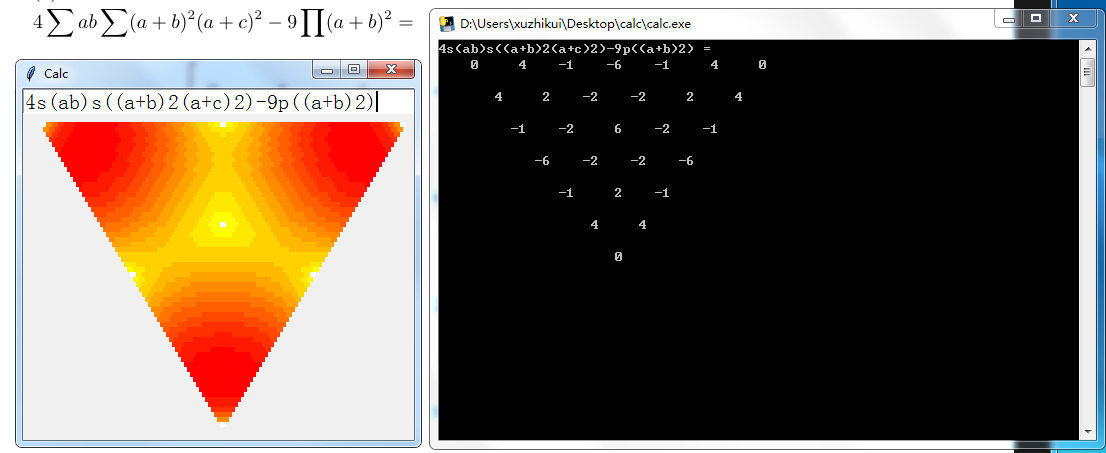
\includegraphics[width=0.85\linewidth]{002}
\end{center}
$ s() $表示sum轮换和,$ p() $表示prod轮换积\\
“前有数字后有字母”会补乘号,如“9/4ab”指$ \dfrac{9}{4}ab $,为避免误解可以写成“9ab/4”\\
要注意的是只能输入齐次式,否则无法运行。\\
一些情况下$ * $和\^{}可省略(\^{}前面是字母或者右括号的话\^{}可省)
\begin{center}
	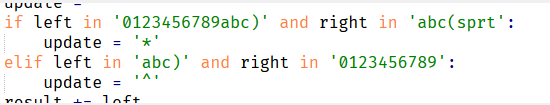
\includegraphics[width=0.5\linewidth]{003}
\end{center}
那么再讲一下怎么取等(或者找反例)\\

取值器的判定是在$ a+b+c=60 $的条件下算的值,中心就是$ (a,b,c)=(20,20,20) $,左上角顶点就是$ (a,b,c)=(60,0,0) $,一般地,到相应字母对边的距离就是其取值(可以发现每边正好60个格子),颜色则代表取值正负:白色为0,红色为正,蓝色为负。一般的,没有蓝色则恒非负,除非题目很ex导致60的精度不够,但是有蓝色就说明一定不是恒非负的,白色自然就是不等式的取等条件。
\subsection{}
有没有可能存在着直接判断一个系数阵是否大于零的粗暴办法呢?\\
拉乘,吴消元法,代数数运算。\\
那么得到的方程必定可以消去两个元变成一元多项式方程,这时候次数可能非常大,没法求根式解。但实际上我们是可以直接对“xxxxx方程的根”作各种运算的,这个过程的感觉就比如得到“xxxx方程的根”的平方等于“xxxxxxxx方程的根”,所以理论上我们可以表示出拉乘所得方程的所有解,只不过那时会是“a=xxxxxxxxxxx(一个超长的整系数方程)的解”这个样子。那么对这些可疑极值点回代计算即可,但你也该意识到这个过程有多离谱了,这确实是个通法,但不是一个好的判定方法。
\subsection{sostool}
配方器\href{https://www.mit.edu/~parrilo/sostools/}{sostool链接}这个需要matlab环境支持
\newpage
\section{二元系数组}
\subsection{杨辉三角}
我们先从杨辉三角说起,姑且默认大家都知道杨辉三角。
\subsection{定义}
我们已经知道了杨辉三角,杨辉三角本身其实就暗示了“一排数字可以和一个二元齐次多项式相对应”。\\
比如$ [1] $对应$ 1 $,$ [1,1] $对应$ a+b $,$ [1,2,1] $对应$ a^{2}+2ab+b^{2} $……依此类推,那么自然地
$$[1,0,2]_{a, b}=a^{2}+2 b^{2}$$
于是我们作这样的记号,类似$ [1,0,2] $的叫做二元系数组
\subsection{二元系数组的运算性质}
下面我们来观察感受一下系数组的运算性质:\\
其实大家学多项式乘法竖式的时候应该对这种运算方式有所了解,比如$ [1,1]$ × $[1,0,0,1]=[1,1,0,1,1] $,这其实可以利用乘法分配律,也就是$ [1,1]$ × $[1,0,0,1]=[1,1]$ × $[1,0,0,0]+[1,1]$ × $[0,0,0,1]=[1,1,0,0,0]+[0,0,0,1,1]=[1,1,0,1,1] $,考虑到他和多项式同构所以系数组可以有分配律,\\
再例如:
$[1,2,3] \times[1,0,1]=[[1,2,3], 0,[1,2,3]]=[1,2,4,2,3]$,或者我们可以这么理解:
\begin{center}
	\begin{tabular}{ccccc}
		&  & 1 & 2 & 3 \\
		1& 2 & 3 &  &  \\
		\hline
		1& 2 & 4 & 2 & 3 \\
	\end{tabular}
\end{center}
$[1,2,3] \times[1,2,3]=[1 \times[1,2,3], 2 \times[1,2,3], 3 \times[1,2,3]]=[1,4,10,12,9]$或者
\begin{center}
	\begin{tabular}{ccccc}
		
		&  & 3 & 6 & 9 \\
		& 2 & 4 & 6 &  \\
		1& 2 & 3 &  &  \\
		\hline
		1& 4 & 10 & 12 & 9 \\
	\end{tabular}
\end{center}
可以发现,系数组(多项式)的乘法,和正整数竖式乘法的区别就是系数组的运算不进位。
\section{系数阵}
\subsection{定义}
把系数组变成三元的,就是系数阵,我们把下面这个东西叫做三元系数阵,设这个东西第一行有$ n+1 $个数,则称它是$ n $阶的。和上面的二元情形类似,它和三元齐次式之间一一对应。左上角的数对应$ a^n $系数,右上角对应$ b^n $系数,下角对应$ c^n $系数,三元齐次式写成这个样子的主要好处就是,使得我们不用写$ a^{3}b^{2}c $之类的东西了,只需要书写系数,这会使得我们更加便于观察一个三元齐次式的结构。

\renewcommand*{\arraystretch}{1.732}\[\left[\begin{matrix}
	x_{00}& & x_{01}& & x_{02} & & \cdots&&  x_{0n}\\
	& x_{10}& & x_{11}& &\cdots&& \begin{sideways}$\ddots$\end{sideways}& \\
	& & x_{20}& &\cdots&& \begin{sideways}$\ddots$\end{sideways}& & \\
	& & & \ddots&& \begin{sideways}$\ddots$\end{sideways} & & & \\
	& & & & x_{n0}& &&& \\
\end{matrix}\right]\]
或者把它倒过来,左下角对应$ a^n $系数,右下角对应$ b^n $系数,上角的数对应$ c^n $系数。
\renewcommand*{\arraystretch}{1.732}\[\left[\begin{matrix}
	& & &&  x_{n0}& && & \\
	& & &\begin{sideways}$\ddots$\end{sideways}& & \ddots&& & \\
	& & x_{20}& & \cdots&&\ddots& & \\
	& x_{10}& & x_{11}&&\cdots& & \ddots& \\
	x_{00}& & x_{01}& & x_{02} & &\cdots&& x_{0n}\\
\end{matrix}\right]\]
例如:$ a+b+c= $
\renewcommand*{\arraystretch}{1.732}\[\left[\begin{matrix}
	1& &1 \\
	& 1&\\
\end{matrix}\right]\]

$ a+2b+3c= $
\renewcommand*{\arraystretch}{1.732}\[\left[\begin{matrix}
	1& &2 \\
	& 3& \\
\end{matrix}\right]\]
$ a^{3}+2b^{3}+3a^{2}b+4c^{3}= $
\renewcommand*{\arraystretch}{1.732}\[\left[\begin{matrix}
	1& & 3& & 0& &2 \\
	& 0& &0 & &0 & \\
	& & 0& &0 & & \\
	& & & 4& & & \\
\end{matrix}\right]\]
$ a^{3}b^{2}c= $
\renewcommand*{\arraystretch}{1.732}\[
\left[\begin{matrix}
	\begin{tabular}{ccccccccccccc}
		0& &0& &0& &0& &0& &0& &0\\
		&0& &0& &1& &0& &0& &0&\\
		& &0& &0& &0& &0& &0& &\\
		& & &0& &0& &0& &0& & &\\
		& & & &0& &0& &0& & & &\\
		& & & & &0& &0& & & & &\\
		& & & & & &0& & & & & &\\
	\end{tabular}
\end{matrix}\right]
\]\\
你会发现,这个“1”在$ a $角的方向上距离边的距离是$ 3 $,
$ bc $同理,每个数所处的坐标和指数向量是对应的,用的就是齐次坐标的规则。
$ a^{3}+2b^{3}+3a^{2}b+4c^{3}= $
\subsection{系数阵的运算}

首先要知道的是一个系数阵乘一个单项系数阵的规律,比如系数阵$ 3 $阶乘$ 3 $阶结果是$ 6 $阶。\\
现在我们把上面两个阵相乘,大家应该能看出发生了什么
\begin{center}
	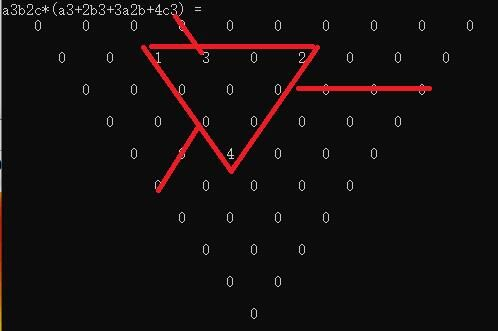
\includegraphics[width=0.7\linewidth]{03}
\end{center}
于是我们来看看这个写法对于三元齐次多项式的乘法带来了怎样一些便利,比方说,三元的杨辉三角现在$ (a+b+c)^{3} $已经有了,我们如何计算$ (a+b+c)^{4} $
\begin{center}
	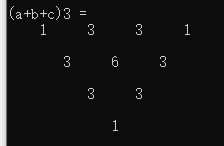
\includegraphics[width=0.4\linewidth]{04}
\end{center}
类似二元系数组,我们可以想象把$ (a+b+c)^{3} $分别乘上$ a,b,c $然后叠加起来,其实就是系数组的叠加原理拓展到三元了。
\begin{center}
	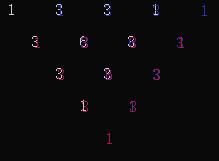
\includegraphics[width=0.3\linewidth]{05}
\end{center}
或者
\begin{center}
	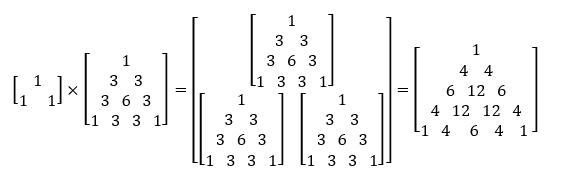
\includegraphics[width=0.6\linewidth]{06}
\end{center}
补充解释:你要想想一块披萨上面的料也全是披萨,前面我称为$ \triangle  a$后面我称为$\triangle b $,那么$ \triangle a×\triangle b $的意思是,把$\triangle b $看成一块披上,每一个非$ 0 $的地方都是料,而这块料是$ \triangle a $这个披萨\\
如果我们直接去思考“最后的这些数由何而来”,就可以这样算出来:
\begin{center}
	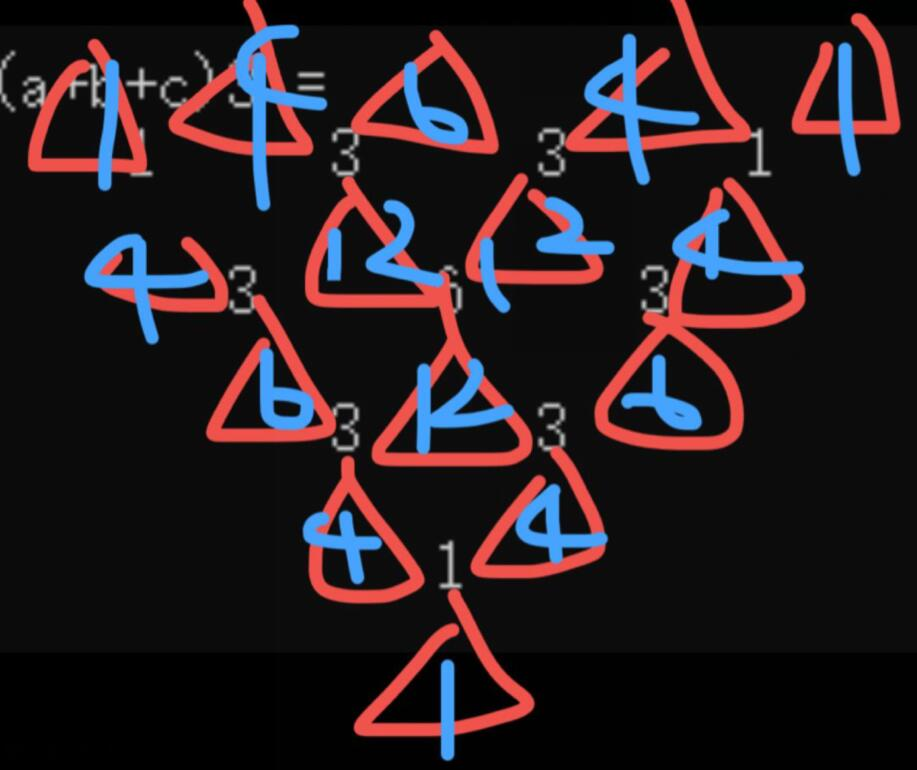
\includegraphics[width=0.27\linewidth]{07}
\end{center}
这也正是杨辉三角的思路在三元情形下的推广,由此我们可以看出,系数阵在“乘以$ (a+b+c) $”这个操作上是带来便利的,此外系数阵还有一个便利,在作轮换和的时候也带来方便。比如说我们把$ (a+b+c)^{3}(a+b+c) $视作$ \displaystyle \sum((a+b+c)^{3}a) $ ,$ (a+b+c)^{3}a $就是
\begin{center}
	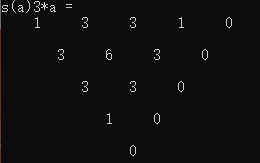
\includegraphics[width=0.31\linewidth]{08}
\end{center}
$ a $角方向加一排$ 0 $,对这个式子作轮换和的话,我们只需要盯着旋转对称的位置相加就行
大体像这个样子,剩下的地方可以直接根据对称性写出来,这里体现的是系数阵在轮换和操作上带来的便利。

\begin{center}
	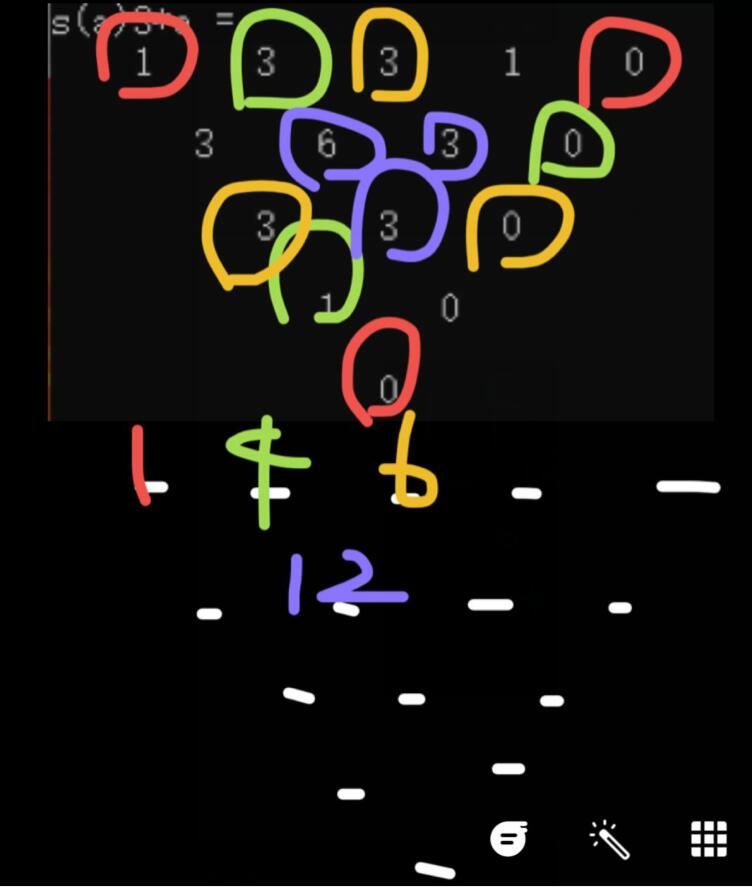
\includegraphics[width=0.35\linewidth]{09}
\end{center}
值得一提的是,如果知道结果是轮换的或轮换对称的,就可以只关注一部分位置上的系数了,此外$ \prod (a-b) $、$ \prod (a+b) $、$\prod (a-b)^{2} $、$ \prod (a+b)^{2} $不难背出来,特别是$ \prod (a-b)^{2} $很有必要背出来,是个很强的结构,记得注意一个多项式被$ a-b $整除的话每行总和都是$ 0 $,对称位置直接写,意思就是不要把整个复制成三份叠起来,这样不好想象,而是去找每一项的来源,这样就可以从被乘的阵上直接读了,乘$ \displaystyle \sum a $、$ \displaystyle \sum ab $、$ \displaystyle \sum a^{2} $之类的都可以用这个技巧,$ a+b $也可以\\
$ \prod (a-b)=\left[\begin{matrix}
	0& &-1& &1& &0\\
	&1& &0& &-1&\\
	& &-1& &1& & \\
	& & &0& & &\\
\end{matrix}\right] $
$ \prod (a+b)= \left[\begin{matrix}
	0& &1& &1& &0\\
	&1& &2& &1&\\
	& &1& &1& & \\
	& & &0& & &\\
\end{matrix}\right]$\\
$\prod (a-b)^{2}=
\left[\begin{matrix}
	\begin{tabular}{ccccccccccccc}
		0& &0& &1& &-2& &1& &0& &0\\
		&0& &-2& &2& &2& &-2& &0&\\
		& &1& &2& &-6& &2& &1& &\\
		& & &-2& &2& &2& &-2& & &\\
		& & & &1& &-2& &1& & & &\\
		& & & & &0& &0& & & & &\\
		& & & & & &0& & & & & &\\
	\end{tabular}
\end{matrix}\right]$\\
$\prod (a+b)^{2}=
\left[\begin{matrix}
	\begin{tabular}{ccccccccccccc}
		0& &0& &1& &2& &1& &0& &0\\
		&0& &2& &6& &6& &2& &0&\\
		& &1& &6& &10& &6& &1& &\\
		& & &2& &6& &6& &2& & &\\
		& & & &1& &2& &1& & & &\\
		& & & & &0& &0& & & & &\\
		& & & & & &0& & & & & &\\
	\end{tabular}
\end{matrix}\right] $
\subsection{习题}
\noindent (1)用系数阵计算$ (a+b)^{2}·(a+c)^{2} $,观察结果形式的特点\\
(2)如何用系数阵计算$ P(a,b,c)×(ab+ac+bc) $,当然$ P(a,b,c) $齐次\\
(3)如何用系数阵计算轮换对称和\\
(4)用系数阵方法将Iran96不等式通分\\
习题2的话,乘$ (ab+ac+bc) $和乘$ (a+b+c) $差不多,比如要计算这个东西乘$ (ab+ac+bc) $的话,可以在心里画这样一些倒三角求和,蓝色的就是积了。
\begin{center}
	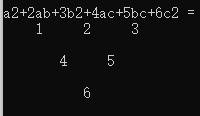
\includegraphics[width=0.35\linewidth]{10}
\end{center}
\begin{center}
	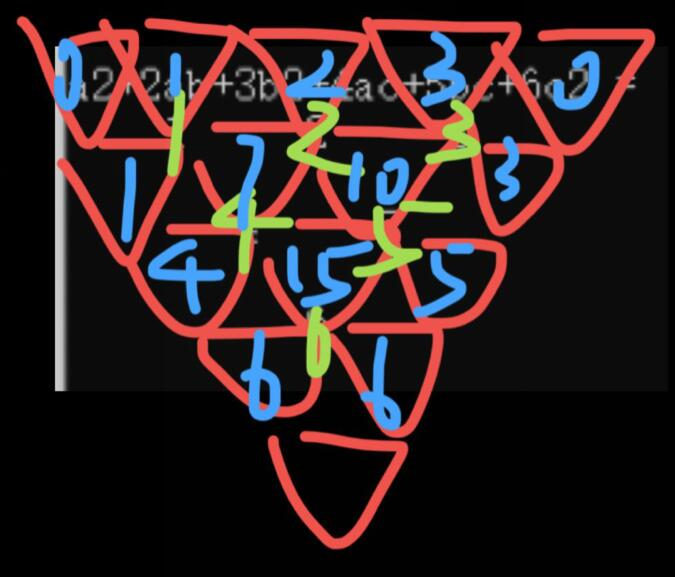
\includegraphics[width=0.35\linewidth]{11}
\end{center}
\section{简单均值不等式}
这里我们只探讨【对于若干系数为1的单项式使用AM-GM不等式】的特点
\subsection{简单的均值不等式}
我们可以先观察几个例子,首先对于$ a^{2}+b^{2}\geq2ab $,即$ a^{2}+b^{2}-2ab\geq0 $
我们知道,$ a^{2}+b^{2}-2ab= $
\renewcommand*{\arraystretch}{1.732}\[\left[\begin{matrix}
	1& & -2& &1 \\
	& 0& &0 & \\
	& & 0& & \\
\end{matrix}\right]\]
$ a^{2}+c^{2}-2ac $的话就是转一下
\renewcommand*{\arraystretch}{1.732}\[\left[\begin{matrix}
	1& & 0& &0 \\
	& -2& &0 & \\
	& & 1& & \\
\end{matrix}\right]\]
那在找个次数高点的例子,$ a^{4}+b^{2}c^{2}-2a^{2}bc= $
\renewcommand*{\arraystretch}{1.732}\[\left[\begin{matrix}
	1& & 0& &0& & 0& &0\\
    & 0& & -2&&0 & & 0&\\
    & & 0& &0& & 1& &\\
    & & & 0&& 0& & &\\
    & & & &0& & & &\\
\end{matrix}\right]\]
到这里其形状的规律已经很明显了,就是“两个$ 1 $以及其中点处的$ -2 $”,实际上根据系数阵的定义很容易验证这一点。\\
顺便补充:如果$ ab $质心不在$ x $上,类似$[a,x,0,b] $,那就是$ (a/2)x^{3}+(a/2)x^{3}+b $均一下。\\
那么再看看三元的情形\\
$ a^{3}+b^{3}+c^{3}-3abc= $
\renewcommand*{\arraystretch}{1.732}\[\left[\begin{matrix}
	1& & 0& &0& & 1\\
	& 0& & -3& &0 &\\
	& & 0& &0& & \\
	& & & 1& & &\\
\end{matrix}\right]\]
这个的证明其实也可以用常用恒等式:\\
$ a^{3}+b^{3}+b^{3}-3 abc=(a+b+c)(a^{2}+b^{2}+c^{2}-ab-ac-bc) $\\
顺便后面这个可以再分解$ (a+b+c)(a+\omega b+\omega ^{2}c)(a+\omega ^{2} b+\omega c) $(和系数阵更没关系了)\\
也可以用sos证明,后面讲到sos会有\label{1}\pageref{2}\\
$ a^{2}b+b^{2}c+c^{2}a-3abc= $
\renewcommand*{\arraystretch}{1.732}\[\left[\begin{matrix}
	0& & 1& &0& & 0\\
	& 0& & -3& &1 &\\
	& & 1& &0& & \\
	& & & 0& & &\\
\end{matrix}\right]\]
$ a^{2}b+ab^{2}+c^{3}-3abc= $
\renewcommand*{\arraystretch}{1.732}\[\left[\begin{matrix}
	0& & 1& &1& & 0\\
	& 0& & -3& &0 &\\
	& & 0& &0& & \\
	& & & 1& & &\\
\end{matrix}\right]\]
我们可以惊讶地发现,其形态就是“三个$ 1 $以及其重心处的$ -3 $”,同理$ n $元的情况也是如此,应当是“$ n $个$ 1 $以及其重心处的$ -n $”
那么这里作一个小补——这些$ 1 $可以有部分重合的,比如\\
$ a^{3}+a^{3}+b^{3}-3a^{2}b= $
\renewcommand*{\arraystretch}{1.732}\[\left[\begin{matrix}
	2& & -3& &0& & 1\\
	& 0& & 0& &0 &\\
	& & 0& &0& & \\
	& & & 0& & &\\
\end{matrix}\right]\]

对应的就是重合的两个$ 1 $和另一个$ 1 $与这三点重心上的$ -3 $

这个大家应该不难接受,那么我们来看一个简单的例子吧
$$
\begin{gathered}
	a, b, c \geq 0, \quad \text { 求证: } \sum a^{5}+2 \sum a^{2} b^{2} c \geq 3 \sum a^{3} b c
\end{gathered}
$$
\begin{center}
	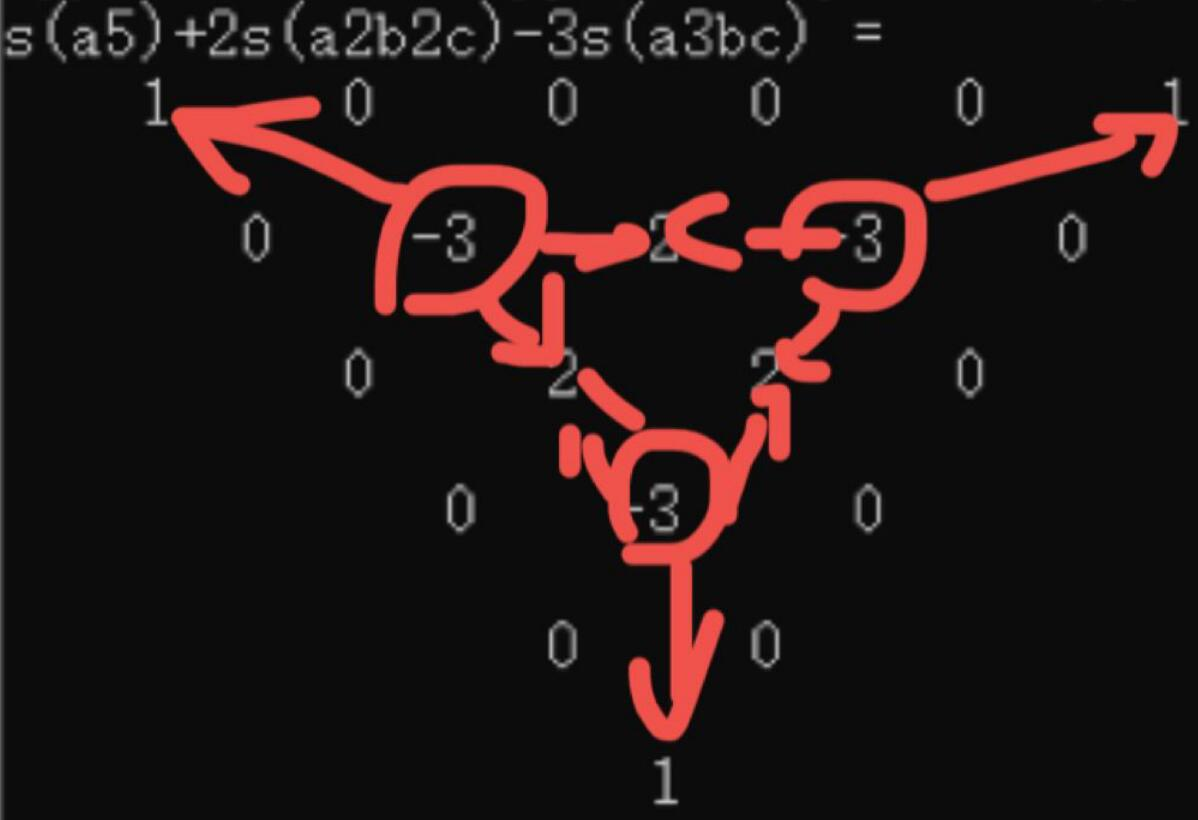
\includegraphics[width=0.4\linewidth]{12}
\end{center}

我们只需看看负项,找找让哪些正项来对付就行,里应外合。下一个例子

$$ a, b, c \geq 0, \quad \text { 求证: } \sum a^{3} b \geq \sum a^{2} b c
$$

接下来我们有两种做法,法一比较容易想到,把它拆成三组$ [1,-2,1] $,每一个$ -1 $拆成$ 1 $和$ -2 $\\
$ \displaystyle \sum (a^{3} b-a^{2} b c)= $
\renewcommand*{\arraystretch}{1.732}\[\left[\begin{matrix}
	0& &1& &0& &0& &0\\
	&0& &-1& &-1& &1&\\
	& &0& &-1& &0& &\\
	& & &1& &0& & &\\
	& & & &0& & & &\\
\end{matrix}\right]\]
换言之也就是:\\
\begin{center}
	注意到$ \displaystyle \sum a^{3} b-\displaystyle \sum a^{2} b c=\displaystyle \sum b c(a-b)^{2} \geq 0 $得证
	这里注意要学会如何把系数阵化为“配方”。
\end{center}
那么再看一个比较通用的法二
$ \Box a^{3} b+\Box b^{3} c+\Box c^{3} a \geq \Box a^{2} b c $
我们不难想象可以通过均值凑出这样的一个局部,而且我们可以用待定系数法解出来,实际上这个系数是4,1,2,
$ 4a^{3}b+b^{3}c+2c^{3}a-7a^{2}bc= $\\
\renewcommand*{\arraystretch}{1.732}\[\left[\begin{matrix}
	0& &4& &0& &0& &0\\
	& 0& &-7& &0& &1&\\
	& &0& &0& &0& &\\
	& & &2& &0& & &\\
	& & & &0& & & &\\
\end{matrix}\right]\]
那么接下来介绍一下在系数阵里如何快速地凑出这三个数,假定我们还不知道它应该是4,1,2。设之为$ p,q,r $,中间那个自然得是$ -(p+q+r) $,我们要保证的是处于$ a^{3}b $及其轮换位置上的、质量$ p,q,r $的三个质点其质心在$ a^{2}bc $的位置上。这其实就是奔驰定理(或拉密定理)

\begin{center}
	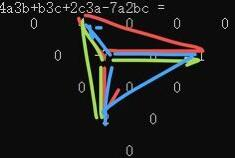
\includegraphics[width=0.4\linewidth]{13}
\end{center}

也就是说这三个系数之比应当等于这三块的面积比,不妨绿色那块面积是1,于是显见红色是2、蓝色是4,这样就直接凑出来啦,这里建议熟悉$ S=\displaystyle \dfrac{1}{2}ab  \sin \theta $
。事实上,此处也可以结合皮克定理,数“有多少个180°”,面积比等于度数比,仅限格点定点的多边形。如下面这个例子:\\
$ \displaystyle  \sum a^{3} b^{2} \geq \displaystyle  \sum a^{2} b^{2} c $

\begin{center}
	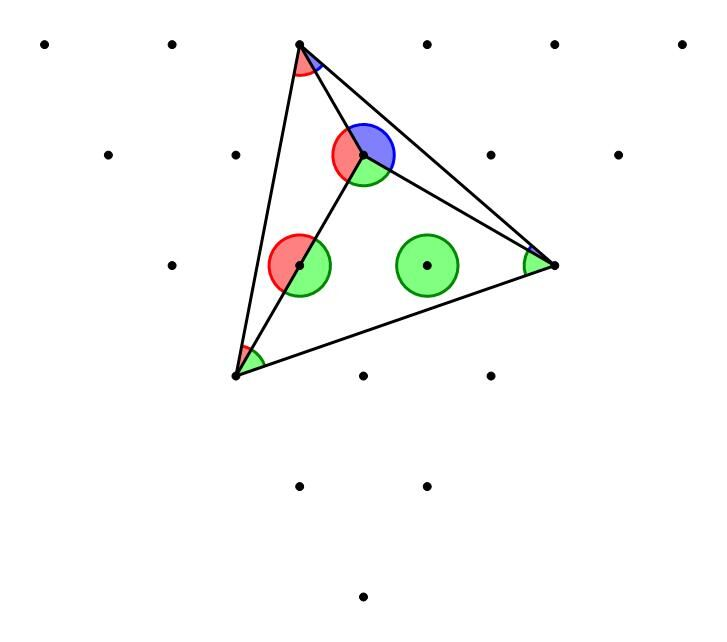
\includegraphics[width=0.4\linewidth]{14}
\end{center}

再看一个均值:$ \displaystyle  \sum a^{5}b^{2}-\displaystyle  \sum a^{3}b^{3}c= $
\renewcommand*{\arraystretch}{1.732}\[\left[\begin{matrix}
	\begin{tabular}{ccccccccccccccc}
		0& &0& &1& &0& &0& &0& &0& &0\\
		&0& &0& &0& &-1& &0& &0& &0&\\
		& &0& &0& &0& &0& &0& &1& &\\
		& & &0& &-1& &0& &-1& &0& & &\\
		& & & &0& &0& &0& &0& & & &\\
		& & & & &1& &0& &0& & & & &\\
		& & & & & &0& &0& & & & & &\\
		& & & & & & &0& & & & & & &\\
	\end{tabular}
\end{matrix}\right]\]


于是其实我们已经暗中得到了一个结论:如果三个$ 1 $和三个$ -1 $构成的正三角形共中心,且$ 1 $的套住$ -1 $的,那么这个非负性成立,证明的话直接根据奔驰定理给出三个均值局部即可。米尔黑德定理就和它类似,如果一个轮换对称六边形套住另一个,那么非负性成立,以上说的都是观察手段,当然不要在解答过程里这样推理,上面这种的话写三个均值相加,或者直接$ (\displaystyle \sum a^{2}b^{2}-\displaystyle \sum a^{4}b^{2}c) $。
这是米尔黑德的例子:
\begin{center}
	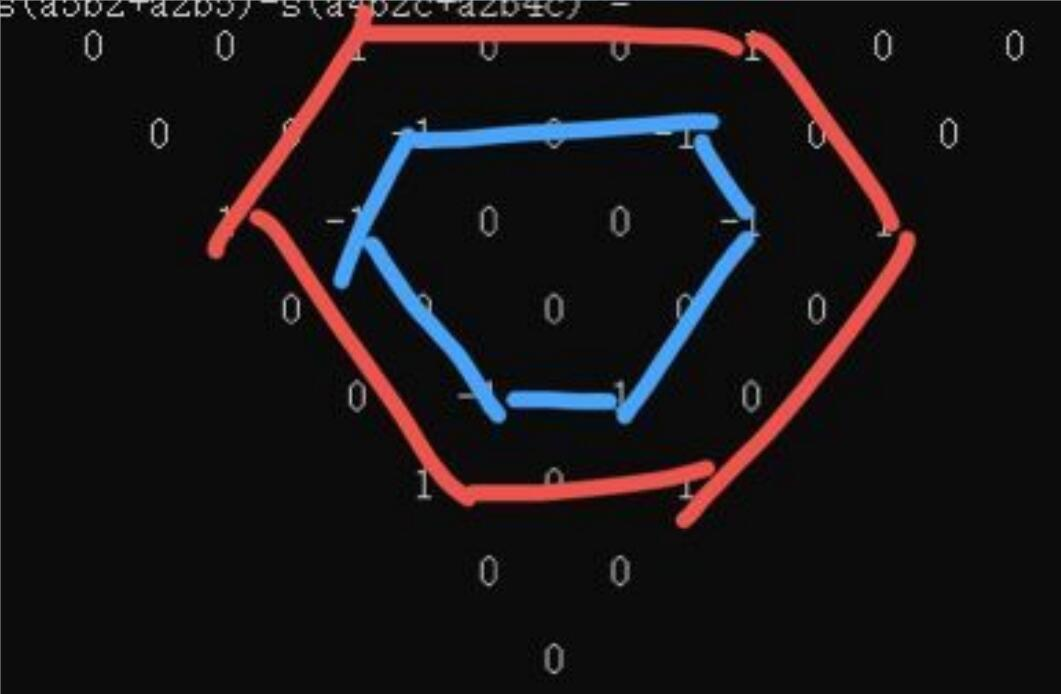
\includegraphics[width=0.45\linewidth]{16}
\end{center}
以上两个结论(正三角形的、“轮换对称六边形”的)事实上暗示了一个道理,靠外的项更贵,靠内的项更贱,就是说在外面的项可以轻易地大过里面的,因此靠外的负项应当小心处理、优先处理,靠外的正项应该尽可能有效利用。\\
\section{两个结构}
\subsection{$ (a-b)^{2n}$结构}
如$ (a-b)^{4} $、$ (a-b)^{6} $这类,在分拆中使用这样的结构可以更有效地利用靠外的正项,比如我们对比一下,如果是用$ (a-b)^{4} $,得到的就是这样
$ (a-b)^{4}= $
\renewcommand*{\arraystretch}{1.732}\[\left[\begin{matrix}
	1& &-4& &6& &-4& &1\\
	&0& &0& &0& &0&\\
	& &0& &0& &0& &\\
	& & &0& &0& & &\\
	& & & &0& & & &\\
\end{matrix}\right]\]
可以理解为拿1个$ a^{4} $、1个$ b^{4} $、6个$ a^{2}b^{2} $解决了4个$ a^{3}b $和4个$ ab^{3} $但如果是用均值做类似的事

$ (a-b)^{2}(a^{2}+b^{2})= $
\renewcommand*{\arraystretch}{1.732}\[\left[\begin{matrix}
	1& &-2& &2& &-2& &1\\
	&0& &0& &0& &0&\\
	& &0& &0& &0& &\\
	& & &0& &0& & &\\
	& & & &0& & & &\\
\end{matrix}\right]\]
就变成拿$ 1 $个$ a^{4} $、$ 1 $个$ b^{4} $、$ 2 $个$ a^{2}b^{2} $解决了$ 2 $个$ a^{3}b $和2个$ ab^{3} $
如果带着靠外项更贵的心态来看,显然上面的性价比更高,况且实际上它们作差就是$ 2ab(a-b)^{2} $,所以显然$ (a-b)^{4} $更紧一些,这里应当感受的是$ n $为不小于$ 2 $的正整数时$ (a-b)^{2n} $比均值紧很多,而且$ n $越大越紧。这只是考虑用$ a^{4} $、$ b^{4} $、$ a^{2}b^{2} $去攻击$ a^{3}b $和$ ab^{3} $
那就近的话自然就是这两组均值\\
\subsection{“1...-1...-1...1”结构}
观察$ (a^{3}-b^{3})(a^{4}-b^{4})$:
\renewcommand*{\arraystretch}{1.732}\[
\left[\begin{matrix}
	\begin{tabular}{ccccccccccccccc}
		1& &0& &0& &-1& &-1& &0& &0& &1\\
		&0& &0& &0& &0& &0& &0& &0&\\
		& &0& &0& &0& &0& &0& &0& &\\
		& & &0& &0& &0& &0& &0& & &\\
		& & & &0& &0& &0& &0& & & &\\
		& & & & &0& &0& &0& & & & &\\
		& & & & & &0& &0& & & & & &\\
		& & & & & & &0& & & & & & &\\
	\end{tabular}
\end{matrix}\right]
\]
我们知道$ (a^{m}-b^{m})(a^{n}-b^{n})$是非负的,形状为对称的“$ 1 $…$ -1 $…$ -1 $…$ 1 $”,其证明只需分$ a\ge b $和$ a<b $两种情况讨论,那么它在系数阵中的规律就是“$ m,n $的值对应其中一个 “$-1$” 到两边的距离”。
\subsection{习题}
*这些习题并不是都能用这节讲到的方法解决,对于搞不定的可以思考能如何投机取巧
$(1) \displaystyle  \sum a^{2} \geq \displaystyle \sum a b \\
(2)  \displaystyle \sum a^{3} \geq \displaystyle \sum a^{2} b \\
(3)  \displaystyle \sum a^{3} b \geq \displaystyle \sum a^{2} b c \\
(4)  \displaystyle \sum a^{5}+2  \displaystyle \sum a^{2} b^{2} c \geq 3  \displaystyle \sum a^{3} b c \\
(5) \displaystyle \sum a^{4}+3 \displaystyle \sum a^{2} b^{2} \geq 2 \displaystyle \sum a b\left(a^{2}+b^{2}\right) \\
(6)  \displaystyle \sum a^{5}+5  \displaystyle \sum a^{3} b^{2} \geq 6  \displaystyle \sum a^{3} b c \\
(7)  \displaystyle \sum a^{5}+3 \displaystyle \sum a^{2} b^{2} c \geq 4  \displaystyle \sum a^{3} b c \\
(8)  \displaystyle \sum a^{5}+8 \displaystyle \sum a^{3} b^{2} \geq 9 \displaystyle \sum a^{3} b c \\
(9)  \displaystyle \dfrac{\displaystyle \sum a^{2} \displaystyle \sum a^{3}}{3 a b c} \geq 4 \displaystyle \sum a^{2}-3 \displaystyle \sum a b \\
(10)  \displaystyle \sum a^{5}+10  \displaystyle \sum a^{3} b^{2} \geq 11  \displaystyle \sum a^{3} b c \\ $
\\
$(1)\dfrac{1}{2} \displaystyle \sum (a-b)^{2}$\\
(2)aab配\\
$(5)(a-b)^{2}(a-c)^{2}$,同时它也等于$\dfrac{1}{2} \displaystyle \sum (a-b)^{4}$
其实这个更容易想到,因为看系数阵的话只有外边一圈,容易想到是不是能分成三条边处理\\
(6)恰好就是三个均值,这里可以利用面积配系数,很明显张成的三块面积$1:2:3$
   \begin{center}
   	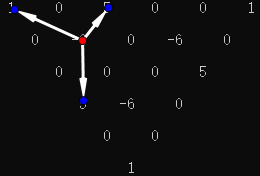
\includegraphics[width=0.5\linewidth]{18}
   \end{center}
(7)可以发现它是(4)的加强,而(4)我们是拆成三个均值完成的,可见相同的方法将失效,把这样几个平方相乘的话强度会增加,可见$\displaystyle \sum a(a-b)^{2}(a-c)^{2}$会是一个比较强的结构,\\
实际上拆下这个$\displaystyle \sum a(a-b)^{2}(a-c)^{2}$之后剩这些:\\
 $\displaystyle \sum (a^{5}+3a^{2}b^{2}c-4a^{3}bc)-\displaystyle \sum (a(a-b)^{2}(a-c)^{2})=$\\
 \renewcommand*{\arraystretch}{1.732}\[\left[\begin{matrix}
 	\begin{tabular}{ccccccccccccc}
 		0& &2& &-1& &-1& &2& &0\\
 		&2& &-8& &6& &-8& &2&\\
 		& &-1& &6& &6& &-1& &\\
 		& & &1& &-8& &-1& & &\\
 		& & & &2& &2& & & &\\
 		& & & & &0& & & & &\\
 	\end{tabular}
 \end{matrix}\right]\]
实际上和$ (a-b)^{2}(a-c)^{2} $的强度差不多,所以如果不是形状特别适合$ (a-b)^{2}(a-c)^{2} $的话一般先从$ (a-b)^{2n} $这个东西试起,如此一来计算量会小一些,说回这个,中间那几个$-8$和$+6$
  \begin{center}
  	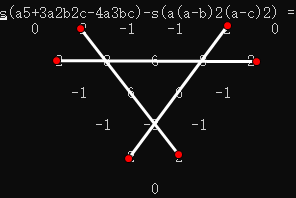
\includegraphics[width=0.4\linewidth]{19}
  \end{center}
正好便于我们拆$\displaystyle \sum c(a-b)^{4}$出来,毕竟$\displaystyle \sum c(a-b)^{4}$正好是$[1,-4,6,-4,1]$,然后就剩:\\
  $ \displaystyle \sum (a^{5}+3a^{2}b^{2}c-4a^{3}bc)-\displaystyle \sum (a(a-b)^{2}(a-c)^{2})-\displaystyle \sum (c(a-b)^{4}) = $
  \renewcommand*{\arraystretch}{1.732}\[\left[\begin{matrix}
  	\begin{tabular}{ccccccccccccc}
  		0& &1& &-1& &-1& &1& &0\\
  		&1& &0& &0& &0& &1&\\
  		& &-1& &0& &0& &-1& &\\
  		& & &-1& &0& &-1& & &\\
  		& & & &1& &1& & & &\\
  		& & & & &0& & & & &\\
  	\end{tabular}
  \end{matrix}\right]\]
$ \displaystyle \sum ab(a-b)(a^{2}-b^{2}) $搞定。\\
那么再说说另一种做法
$ \displaystyle \sum (a^{5}+3a^{2}b^{2}c-4a^{3}bc)= $
  \renewcommand*{\arraystretch}{1.732}\[\left[\begin{matrix}
  	\begin{tabular}{ccccccccccccc}
  		1& &0& &0& &0& &0& &1\\
  		&0& &-4& &3& &-4& &0&\\
  		& &0& &3& &3& &0& &\\
  		& & &0& &-4& &0& & &\\
  		& & & &0& &0& & & &\\
  		& & & & &1& & & & &\\
  	\end{tabular}
  \end{matrix}\right]\]
从一开始就考虑靠$ (a-b)^{4} $来发挥里面的3,当然,因为只有3所以拿半个,也就是$ \dfrac{1}{2} \displaystyle \sum c(a-b)^{4} $,于是中间全没了,剩这个:
 \renewcommand*{\arraystretch}{1.732}\[\left[\begin{matrix}
	\begin{tabular}{ccccccccccccc}
		1& &$ -\dfrac{1}{2} $& &0& &0& &$ -\dfrac{1}{2} $& &1\\
		&$ -\dfrac{1}{2} $& &0& &0& &0& &$ -\dfrac{1}{2} $&\\
		& &0& &0& &0& &0& &\\
		& & &0& &0& &0& & &\\
		& & & &$ -\dfrac{1}{2} $& &$ -\dfrac{1}{2} $& & & &\\
		& & & & &1& & & & &\\
	\end{tabular}
  \end{matrix}\right]\]
也就是$ \displaystyle \dfrac{1}{2} \displaystyle \sum (a-b)(a^{4}-b^{4}) $也结束了\\
(8)是(6)的加强,我们可以考虑用$ (a-b)^{4} $来消耗最外面的$ a^5 $,那比方说我们尝试$ \displaystyle \sum a(a-b)^{4} $会导致变成这样:\\
$  \displaystyle \sum (a^{5}+8 a^{3} b^{2}-9a^{3}bc)-\displaystyle \sum a(a-b)^{4}=$
  \renewcommand*{\arraystretch}{1.732}\[\left[\begin{matrix}
  	\begin{tabular}{ccccccccccccc}
  		0& &4& &2& &4& &-1& &0\\
  		&-1& &-9& &0& &-9& &4&\\
  		& &4& &0& &0& &2& &\\
  		& & &2& &-9& &4& & &\\
  		& & & &4& &-1& & & &\\
  		& & & & &0& & & & &\\
  	\end{tabular}
  \end{matrix}\right]\]
这个$ -1 $脱离了正项的凸包,意味着放过头了,这肯定不行了,因此吸取教训(只是演示一下可能的错误)。拆$ \dfrac{1}{2}\displaystyle \sum (a+b)(a-b)^{4} $,这样的话一方面不会出现上面这样的翻车。
  \begin{center}
  	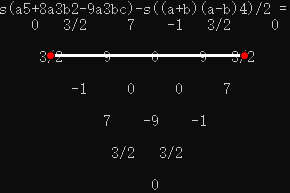
\includegraphics[width=0.4\linewidth]{20}
  \end{center}
另一方面$ a^{4}b $和$ ab^{4} $上系数相等了,便于我们再去拿$ c(a-b)^{4} $,后面计算不说了,顺便我们知道 \\
$ \dfrac{1}{5} \displaystyle \sum (4a+b)(a-b)^{4} $是整系数的\\
$ \dfrac{1}{5} \displaystyle \sum (3a+2b)(a-b)^{4} $\\
$ \dfrac{1}{5} \displaystyle \sum (2a+3b)(a-b)^{4} $\\
$ \dfrac{1}{5} \displaystyle \sum (a+4b)(a-b)^{4} $\\
甚至这几个都是整系数的。
以至于可以搞出$  \displaystyle \sum (a^{5}+8 a^{3} b^{2}-9a^{3}bc)- \displaystyle \sum \dfrac{1}{5}(3a+2b+5c)(a-b)^{4}= $
  \renewcommand*{\arraystretch}{1.732}\[\left[\begin{matrix}
  	\begin{tabular}{ccccccccccccc}
  		0& &1& &6& &0& &0& &0\\
  		&0& &-1& &-6& &-1& &1&\\
  		& &0& &-6& &-6& &6& &\\
  		& & &6& &-1& &0& & &\\
  		& & & &1& &0& & & &\\
  		& & & & &0& & & & &\\
  	\end{tabular}
  \end{matrix}\right]\]
\section{舒尔不等式}
\subsection{舒尔不等式}
$ a,b,c \geq 0,t\in \mathbb{R}\implies a^{t}(a-b)(a-c)+b^{t}(b-c)(b-a)+c^{t}(c-a)(c-b)\geq 0$\\当且仅当$ a=b=c $,或其中两个数相等而另外一个为零时,等号成立。
特别地,当$ t $为非负偶数时,此不等式对任意实数$ a,b,c $成立。\\
证明:由对称性,不妨设$ a\geq b\geq c$,则 $a^{t}-b^{t}+c^{t}\geq 0 $\\
$ a^{t}(a-b)(a-c)+b^{t}(b-c)(b-a)+c^{t}(c-a)(c-b)=a^{t}(a-b)^{2}+(a-b)(a-c)(a^{t}-b^{t}+c^{t})+c^{t}(b-c)^{2}\geq 0 $\\
核心思想就是,把$ a-c $这个大数,拆成$ a-b $和$ b-c $充分利用其非负性\\
我们还要知道像这样的都是schur:\\
$\displaystyle  \sum  a^{m}\left(a^{n}-b^{n}\right)\left(a^{n}-c^{n}\right)$,$\displaystyle \sum b^{m} c^{m}\left(a^{n}-b^{n}\right)\left(a^{n}-c^{n}\right)$\\
当$ t $取$ 0 $时,即$ \displaystyle  \sum a^{2}\geq \displaystyle  \sum ab$,即均值不等式。\\
更多内容请自行查阅资料,百度:\href{https://baike.baidu.com/item/%E8%88%92%E5%B0%94%E4%B8%8D%E7%AD%89%E5%BC%8F/4224241?fr=aladdin}{舒尔不等式}
\begin{center}
	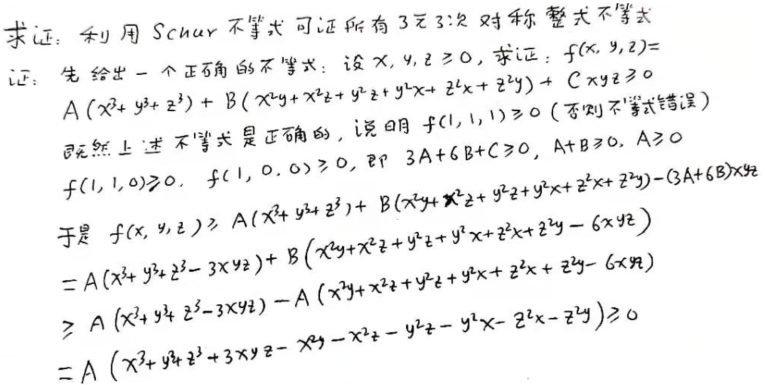
\includegraphics[width=0.8\linewidth]{36}
\end{center}
(平行线\quad 龚固)
\subsection{简单的舒尔不等式}
我们探索到这个阶段,很容易想到一个简单的问题,齐三次的,轮换对称的问题有没有通用的配方办法。考虑到必须有$ F(a,b,0) \geq 0 $,我们容易发现“最强”的问题就是
\renewcommand*{\arraystretch}{1.732}\[\left[\begin{matrix}
	1& &-1& &-1& &1\\
	&-1& &3& &-1&\\
	& &-1& &-1& & \\
	& & &1& & &\\
\end{matrix}\right]\]
这时候我们便要聚焦这个问题,容易发现它是没法靠均值解决的(不升次数的话)。\\
我们知道这个东西叫做舒尔不等式,考虑到它在系数阵里的形状相当有特点,我们便将其引入配方技术之中,毕竟它便于使用,承认这是配方法的一部分就省去了将它特地配方的多余操作。\\
schur在系数阵视角下形状独特,
比如三次的像这样
$ \displaystyle \sum (a(a-b)(a-c))= $
\renewcommand*{\arraystretch}{1.732}\[\left[\begin{matrix}
	1& &-1& &-1& &1\\
	&-1& &3& &-1&\\
	& &-1& &-1& & \\
	& & &1& & &\\
\end{matrix}\right]\]
四次的像这样
$ \displaystyle \sum (a^{2}(a-b)(a-c))= $
\renewcommand*{\arraystretch}{1.732}\[\left[\begin{matrix}
	1& &-1& &0& &-1& &1\\
	&-1& &1& &1& &-1&\\
	& &0& &1& &0& &\\
	& & &-1& &-1& & &\\
	& & & &1& & & &\\
\end{matrix}\right]\]
五次的像这样
$ \displaystyle \sum (a^{3}(a-b)(a-c))= $
\renewcommand*{\arraystretch}{1.732}\[\left[\begin{matrix}
	\begin{tabular}{ccccccccccccc}
		1& &-1& &0& &0& &-1& &1\\
		&-1& &1& &0& &1& &-1&\\
		& &0& &0& &0& &0& &\\
		& & &0& &1& &0& & &\\
		& & & &-1& &-1& & & &\\
		& & & & &1& & & & &\\
	\end{tabular}
\end{matrix}\right]\]
这里规律已经很明显了。再顺便偏个题,schur的一个有趣配方,如果将三次的schur乘上$ (a+b)(a+c)(b+c) $你会惊讶地发现,乘出来的非零项比schur本身还少
\renewcommand*{\arraystretch}{1.732}\[\left[\begin{matrix}
	\begin{tabular}{ccccccccccccc}
		0& &1& &0& &-2& &0& &1& &0\\
		&1& &0& &0& &0& &0& &1&\\
		& &0& &0& &0& &0& &0& &\\
		& & &-2& &0& &0& &-2& & &\\
		& & & &0& &0& &0& & & &\\
		& & & & &1& &1& & & & &\\
		& & & & & &0& & & & & &\\
	\end{tabular}
\end{matrix}\right]\]
结果是这个,不过这个就不要追问为什么了,偶然发现的,高次舒尔就没找到类似的恒等式了。
\begin{1}

证明下式$ \geq 0 $\\
\renewcommand*{\arraystretch}{1.732}\[\left[\begin{matrix}
	\begin{tabular}{ccccccccccccc}
		0&  &1  &  & 0 &  & -2 &  & 0 &  & 1 &  & 0\\
		&1  &  & -2 &  & 1 &  & 1 &  & -2 &  & 1 & \\
		&  & 0 &  & 1 &  &  0&  &  1&  &  0&  & \\
		&  &  &  -2 &  & 1 &  & 1 &  & -2  &  &  & \\
		&  &  &  &  0&  &-2  &  & 0 &  &  &  & \\
		&  &  &  &  &  1&  &1  &  &  &  &  & \\
		&  &  &  &  &  &  0&  &  &  &  &  & \\
	\end{tabular}
\end{matrix}\right]\]
\end{1}
\begin{2}

拿一个$ (a-b)^{2}(a-c)^{2}(b-c)^{2} $出来,
提完会是这样,
\renewcommand*{\arraystretch}{1.732}\[\left[\begin{matrix}
	\begin{tabular}{ccccccccccccc}
		0&  &1  &  & -1 &  & 0 &  & -1 &  & 1 &  & 0\\
		&1  &  & 0 &  & -1 &  & -1 &  & 0 &  & 1 & \\
		&  & -1 &  & -1 &  &  6&  &  -1&  &  -1&  & \\
		&  &  &  0 &  & -1 &  & -1 &  & 0  &  &  & \\
		&  &  &  &  -1&  &0  &  & -1 &  &  &  & \\
		&  &  &  &  &  1&  &1  &  &  &  &  & \\
		&  &  &  &  &  &  0&  &  &  &  &  & \\
	\end{tabular}
\end{matrix}\right]\]
那么$ ab $边上的$ 1,-1,0,-1,1 $暗示了schur:
$$ (x-y)^{2}(x-z)^{2}(y-z)^{2}+\displaystyle \sum x y \cdot \displaystyle \sum x^{2}(x-y)(x-z)+x y z \cdot \displaystyle \sum x(x-y)(x-z) \geq 0 $$
重点是那三个菱形,其它的是0
\begin{center}
	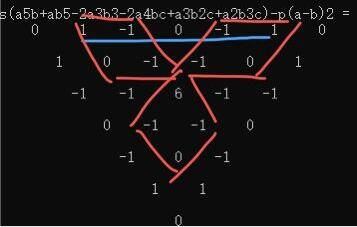
\includegraphics[width=0.5\linewidth]{17}
\end{center}

于是这里就会考虑这个了,这是$ab$Schur$4 $,那么对称的也扣掉,就是$ \displaystyle \sum ab·$ schur $4 $,这样一来最外面一圈就都没了,实际上里面刚好剩下一个三次的schur,那就好了,也就是这样
$ (x-y)^{2}(x-z)^{2}(y-z)^{2}+\displaystyle \sum x y \cdot \displaystyle \sum x^{2}(x-y)(x-z)+x y z \cdot \displaystyle \sum x(x-y)(x-z) \geq 0 $
\\
\end{2}
\subsection{习题}
\noindent (1) $2 \displaystyle  \sum a^{3}+3 a b c \geq 3\displaystyle  \sum  a^{2} b$\\
(2) $2\displaystyle  \sum  a^{4}+\displaystyle  \sum  a^{2} b c \geq 3 \sum a^{2} b^{2}$\\
(3) $ \displaystyle  \sum \dfrac{1}{(a+b)^{2}} \geq \dfrac{9}{4 \displaystyle  \sum a b}$\\
(4) $\displaystyle  \sum  a^{6}+3 a^{2} b^{2} c^{2} \geq 2 \displaystyle  \sum  a^{3} b^{3}$\\
(5) $\displaystyle  \sum a^{5}+\displaystyle  \sum  a^{2} b^{2} c \geq \displaystyle  \sum a^{2} b^{2}(a+b)$\\
(6) $ \displaystyle  \sum  \dfrac{a^{2} b^{2}}{c}+\displaystyle  \sum  a^{3}+6 a b c \geq 2 \displaystyle  \sum  a b(a+b)$\\
(7) $4 \displaystyle  \sum a^{5}+2\sum a^{2} b^{2} c \geq 3 \displaystyle  \sum  a b\left(a^{3}+b^{3}\right)$\\
(8) $\displaystyle  \sum  a^{5}+2  \displaystyle  \sum  a^{2} b^{2} c \geq \displaystyle  \sum  a^{3}\left(b^{2}+b c+c^{2}\right)$\\
(9) $\displaystyle  \sum a^{5}+6  \displaystyle  \sum a^{2} b^{2} c \geq 7 \displaystyle  \sum  a^{3} b c$\\
(10) $21 a b c+\dfrac{a^{5}}{b c} \geq 4\displaystyle  \sum  a b(a+b)$\\
\noindent (1)  \renewcommand*{\arraystretch}{1.732}\[\left[\begin{matrix}
	2& &-3& &0& &2\\
	&0& &3& &-3&\\
	& &-3& &0& & \\
	& & &2& & &\\
\end{matrix}\right]\] 
上次也说明了,仅仅用简单均值不可能利用上中间的3,所以提出一个schur,变成三个$ [1,-2,1] $
 \renewcommand*{\arraystretch}{1.732}\[\left[\begin{matrix}
	1& &-2& &1& &1\\
	&1& &0& &-2&\\
	& &-2& &1& & \\
	& & &1& & &\\
\end{matrix}\right]\]
即$ \displaystyle \sum a(a-b)(a-c)+\displaystyle \sum a^{2}(a-b)\geq 0 $\\
(2)\renewcommand*{\arraystretch}{1.732}\[\left[\begin{matrix}
	2& &0& &-3& &0& &2\\
	&0& &1& &1& &0&\\
	& &-3& &1& &-3& &\\
	& & &0& &0& & &\\
	& & & &2& & & &\\
\end{matrix}\right]\]
一样的道理,要把中间三个1用上,所以拿一份schur,然后也是只需均值\\
$ \displaystyle  \sum (2a^{4}+a^{2}bc-3a^{2}b^{2})-\displaystyle  \sum a^{2}(a-b)(b-c) $
\renewcommand*{\arraystretch}{1.732}\[\left[\begin{matrix}
	1& &1& &-3& &1& &1\\
	&1& &0& &0& &1&\\
	& &-3& &0& &-3& &\\
	& & &1& &1& & &\\
	& & & &1& & & &\\
\end{matrix}\right]\]
即$ \displaystyle \sum a^{2}(a-b)(a-c)+\displaystyle \sum a^{4}+\displaystyle \sum (a^{3}b+ab^{3})\geq \displaystyle \sum a^{2}(a-b)(a-c)+3\displaystyle \sum a^{2}b^{2}$\\
(3)是iran96,化整后变成这样一个六次的问题\\
$ 4\displaystyle \sum ab\displaystyle \sum (a+b)^{2}(a+c)^{2}-9\prod (a+b)^{2}= $
\renewcommand*{\arraystretch}{1.732}\[\left[\begin{matrix}
	\begin{tabular}{ccccccccccccc}
		0& &4& &-1& &-6& &-1& &4& &0\\
		&4& &2& &-2& &-2& &2& &4&\\
		& &-1& &-2& &6& &-2& &-1& &\\
		& & &-6& &-2& &-2& &-6& & &\\
		& & & &-1& &2& &-1& & & &\\
		& & & & &4& &4& & & & &\\
		& & & & & &0& & & & & &\\
	\end{tabular}
\end{matrix}\right]\]
首先我们观察到第一行总和为$ 0 $,即$ F(1,1,0)=0 $,即$ a=b $且$ c=0 $时取等
\begin{center}
	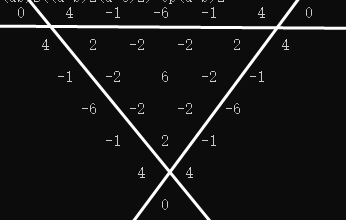
\includegraphics[width=0.4\linewidth]{22}
\end{center}
然后再一看,中间就是一个schur的两倍,故这样分成四块分别解决即可\\
(4)\renewcommand*{\arraystretch}{1.732}\[\left[\begin{matrix}
	\begin{tabular}{ccccccccccccc}
		1& &0& &0& &-2& &0& &0& &1\\
		&0& &0& &0& &0& &0& &0&\\
		& &0& &0& &3& &0& &0& &\\
		& & &-2& &0& &0& &-2& & &\\
		& & & &0& &0& &0& & & &\\
		& & & & &0& &0& & & & &\\
		& & & & & &1& & & & & &\\
	\end{tabular}
\end{matrix}\right]\]
\begin{center}
	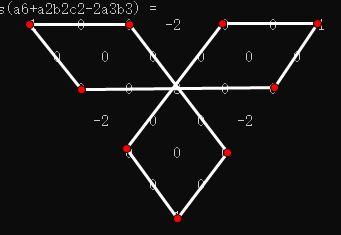
\includegraphics[width=0.5\linewidth]{23}
\end{center}
\begin{center}
	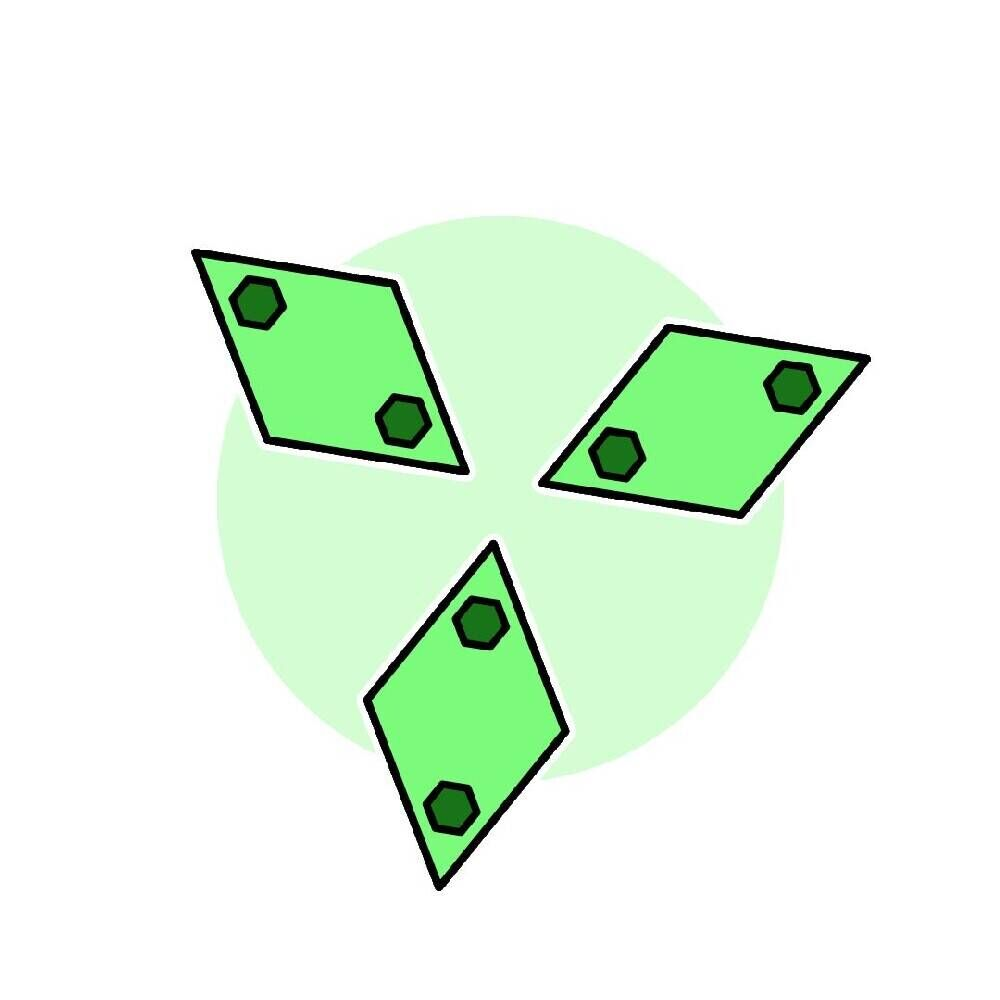
\includegraphics[width=0.4\linewidth]{21}
\end{center}
还是一样的道理,关键在于如何利用中间的3,那么自然地想到这样的schur,也就是减掉$ \displaystyle  \sum a^{2}(a^{2}-b^{2})(a^{2}-c^{2}) $
\renewcommand*{\arraystretch}{1.732}\[\left[\begin{matrix}
	\begin{tabular}{ccccccccccccc}
		0& &0& &1& &-2& &1& &0& &0\\
		&0& &0& &0& &0& &0& &0&\\
		& &1& &0& &0& &0& &1& &\\
		& & &-2& &0& &0& &-2& & &\\
		& & & &1& &0& &1& & & &\\
		& & & & &0& &0& & & & &\\
		& & & & & &0& & & & & &\\
	\end{tabular}
\end{matrix}\right]\]
取出之后剩下三个$ [1,-2,1] $结束\\
即$\displaystyle  \sum  a^{6}+3 a^{2} b^{2} c^{2} \geq \displaystyle  \sum (a^{4}b^{2}+a^{2}b^{4}) \geq 2 \displaystyle  \sum  a^{3} b^{3}$\\
(5)\begin{center}
	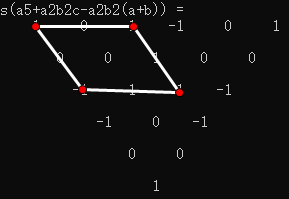
\includegraphics[width=0.5\linewidth]{24}
\end{center}
这是一个舒尔$ \displaystyle  \sum a(a^{2}-b^{2})(a^{2}-c^{2}) $,一共有三个。可以看出即使是像这样的变形,schur在系数阵里依然保持原本的形状规律,这里$ a,b,c $取作$ a^{2},b^{2},c^{2} $,$ t $取$ \dfrac{1}{2} $\\
即$\displaystyle  \sum a^{5}+\displaystyle  \sum  a^{2} b^{2} c -\displaystyle  \sum a^{2} b^{2}(a+b)=\displaystyle  \sum x^{3}(x-y)(x-z)+\displaystyle  \sum x^{2}(y+z)(x-y)(x-z)+\displaystyle  \sum xyz(x-y)(x-z)$\\
(6)\renewcommand*{\arraystretch}{1.732}\[\left[\begin{matrix}
	\begin{tabular}{ccccccccccccc}
		0& &0& &0& &1& &0& &0& &0\\
		&0& &1& &-2& &-2& &1& &0&\\
		& &0& &-2& &6& &-2& &0& &\\
		& & &1& &-2& &-2& &1& & &\\
		& & & &0& &1& &0& & & &\\
		& & & & &0& &0& & & & &\\
		& & & & & &0& & & & & &\\
	\end{tabular}
\end{matrix}\right]\]
这就是两个schur重叠,倒的那个是$ \displaystyle  \sum b^{2}c^{2}(a-b)(a-c) $\\
可以理解为schur定理t=-2\\
$\displaystyle  \sum  b^{2} c^{2}(a-b)(a-c)=a^{2} b^{2} c^{2} \displaystyle  \sum  a^{-2}(a-b)(a-c) $\\
理解为换元也是可以的
$\displaystyle  \sum b^{2} c^{2}(a-b)(a-c)=\displaystyle  \sum b c(b c-a b)(b c-a c)$\\
(7)\renewcommand*{\arraystretch}{1.732}\[\left[\begin{matrix}
	\begin{tabular}{ccccccccccccc}
		4& &-3& &0& &0& &-3& &4\\
		&-3& &0& &2& &0& &-3&\\
		& &0& &2& &2& &0& &\\
		& & &0& &0& &0& & &\\
		& & & &-3& &-3& & & &\\
		& & & & &4& & & & &\\
	\end{tabular}
\end{matrix}\right]\]
提一个4倍schur:$ \displaystyle \sum (4a^{5}+2a^{2}b^{2}c-3ab(a^{3}+b^{3}))-4\displaystyle \sum (a^{3}(a-b)(a-c))= $
\renewcommand*{\arraystretch}{1.732}\[\left[\begin{matrix}
	\begin{tabular}{ccccccccccccc}
		0& &1& &0& &0& &1& &0\\
		&1& &-4& &2& &-4& &1&\\
		& &0& &2& &2& &0& &\\
		& & &0& &-4& &0& & &\\
		& & & &1& &1& & & &\\
		& & & & &0& & & & &\\
	\end{tabular}
\end{matrix}\right]\]
很明显$ 4 $个$ 1 $攻击一个$ -4 $,六个均值,也可以说是三个四元均值\\
那么如果换个思路,为了把$ -3 $弄掉而提$ 3 $倍schur:\\
$ \displaystyle \sum (4a^{5}+2a^{2}b^{2}c-3ab(a^{3}+b^{3}))-3\displaystyle \sum (a^{3}(a-b)(a-c))= $
\renewcommand*{\arraystretch}{1.732}\[\left[\begin{matrix}
	\begin{tabular}{ccccccccccccc}
		1& &0& &0& &0& &0& &1\\
		&0& &-3& &2& &-3& &0&\\
		& &0& &2& &2& &0& &\\
		& & &0& &-3& &0& & &\\
		& & & &0& &0& & & &\\
		& & & & &1& & & & &\\
	\end{tabular}
\end{matrix}\right]\]
剩下就是这样,正好也是均值,重心,三元均值。\\
甚至我们可以提2倍schur,为了用到中间的2,取第五题那样的schur:\\
$ \displaystyle \sum (4a^{5}+2a^{2}b^{2}c-3ab(a^{3}+b^{3}))-
 2\displaystyle \sum a(a^{2}-b^{2})(a^{2}-c^{2})=$
 \renewcommand*{\arraystretch}{1.732}\[\left[\begin{matrix}
 	\begin{tabular}{ccccccccccccc}
 		2& &-3& &2& &2& &-3& &2\\
 		&-3& &0& &0& &0& &2&\\
 		& &2& &0& &0& &-3& &\\
 		& & &2& &0& &2& & &\\
 		& & & &-3& &-3& & & &\\
 		& & & & &2& & & & &\\
 	\end{tabular}
 \end{matrix}\right]\]
然后可以拆成三条$ [1,-3,2,2,-3,1] $,这恰好是$ (a+b)(a-b)^{4}$\\
注:提出的结构必须契合不等式的取等,首先注意到$ ab $边上和为$ 0 $,因此你要动角上那个1的话,不可能用均值或者$ (a-b)^{2n} $,因为它是二元对称的,所以总之先考虑$ (a+b)(a-b)^{4}$这个通常来说最强的东西\\
(8)\renewcommand*{\arraystretch}{1.732}\[\left[\begin{matrix}
	\begin{tabular}{ccccccccccccc}
		1& &0& &-1& &-1& &0& &1\\
		&0& &-1& &2& &-1& &0&\\
		& &-1& &2& &2& &-1& &\\
		& & &-1& &0& &-1& & &\\
		& & & &0& &0& & & &\\
		& & & & &1& & & & &\\
	\end{tabular}
\end{matrix}\right]\]
显然不能提出三个大schur:$ \displaystyle \sum a(a^{2}-b^{2})(a^{2}-c^{2}) $,提完会当场去世。\\
可以试试提$ \displaystyle \sum a^{3}(a-b)(a-c) $:
\renewcommand*{\arraystretch}{1.732}\[\left[\begin{matrix}
	\begin{tabular}{ccccccccccccc}
		0& &1& &-1& &-1& &1& &0\\
		&1& &-2& &2& &-2& &1&\\
		& &-1& &2& &2& &-1& &\\
		& & &-1& &-2& &-1& & &\\
		& & & &1& &1& & & &\\
		& & & & &0& & & & &\\
	\end{tabular}
\end{matrix}\right]\]
看到这个我们顶多想到拆三个小schur,但也会去世。(实际上可以配方,但现在先假装不会)于是我们还有最后一个选择\\
拆三个四阶的schur:
$ \displaystyle \sum  (a^{5}+2a^{2}b^{2}c-a^{3}(b^{2}+bc+c^{2}))-\displaystyle \sum a \displaystyle \sum  a^{2}(a-b)(a-c)=0 $
然后拆完发现啥都没了,拆了三个这样的四阶schur:
\begin{center}
	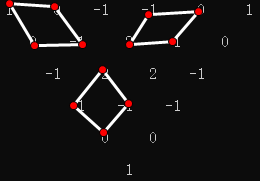
\includegraphics[width=0.4\linewidth]{25}
\end{center}
反正也就这么一个选择,所以有因式$ \displaystyle \sum a $,这提示我们做题时要先因式分解\\
(9)\renewcommand*{\arraystretch}{1.732}\[\left[\begin{matrix}
	\begin{tabular}{ccccccccccccc}
		1& &0& &0& &0& &0& &1\\
		&0& &-7& &6& &-7& &0&\\
		& &0& &6& &6& &0& &\\
		& & &0& &-7& &0& & &\\
		& & & &0& &0& & & &\\
		& & & & &1& & & & &\\
	\end{tabular}
\end{matrix}\right]\]
这是上次均值习题的升级版,提一个schur:
$ \displaystyle \sum (a^{5}+6a^{2}b^{2}c+7a^{3}bc)-\displaystyle \sum a^{3}(a-b)(a-c)= $
\renewcommand*{\arraystretch}{1.732}\[\left[\begin{matrix}
	\begin{tabular}{ccccccccccccc}
		0& &1& &0& &0& &1& &0\\
		&1& &-8& &6& &-8& &1&\\
		& &0& &6& &6& &0& &\\
		& & &0& &-8& &0& & &\\
		& & & &1& &1& & & &\\
		& & & & &0& & & & &\\
	\end{tabular}
\end{matrix}\right]\]
然后是三个[1,-4,6,-4,1]\\
(10)齐次化即$ \displaystyle \sum a^{6}+21a^{2}b^{2}c^{2}-4\displaystyle \sum a^{2}b^{2}(ac+bc)= $
\renewcommand*{\arraystretch}{1.732}\[\left[\begin{matrix}
	\begin{tabular}{ccccccccccccc}
		1& &0& &0& &0& &0& &0& &1\\
		&0& &0& &-4& &-4& &0& &0&\\
		& &0& &-4& &21& &-4& &0& &\\
		& & &0& &-4& &-4& &0& & &\\
		& & & &0& &0& &0& & & &\\
		& & & & &0& &0& & & & &\\
		& & & & & &1& & & & & &\\
	\end{tabular}
\end{matrix}\right]\]
和上一题差不多,一个schur和三个$ [1,-4,6,-4,1] $
\section{配方}
\subsection{平方}
下面分别是$ (a-b)^{2} $、$ (a+b-2c)^{2} $、$ (a+2b-3c)^{2} $,
\renewcommand*{\arraystretch}{1.732}\[\left[\begin{matrix}
	1& &-2& &1\\
	&0& &0&\\
	& &0& &\\
\end{matrix}\right]\]
\renewcommand*{\arraystretch}{1.732}\[\left[\begin{matrix}
	1& &2& &1\\
	&-4& &-4&\\
	& &4& &\\
\end{matrix}\right]\]
\renewcommand*{\arraystretch}{1.732}\[\left[\begin{matrix}
	1& &4& &4\\
	&-6& &-12&\\
	& &9& &\\
\end{matrix}\right]\]
试观察其特点
\begin{center}
	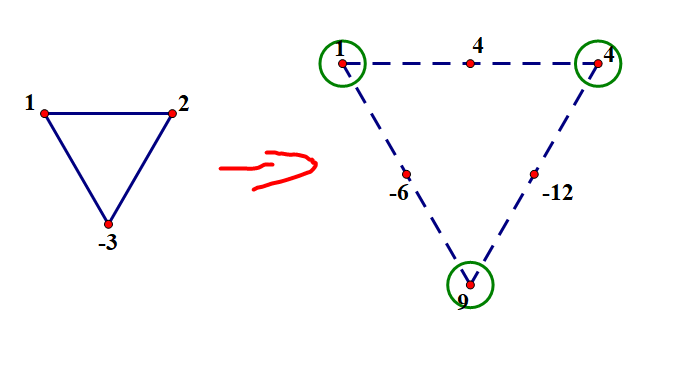
\includegraphics[width=0.5\linewidth]{26}
\end{center}
首先把要平方的阵放大一倍,在对应位置(在大阵上可以称作“桩”)写上小阵各项的平方,然后在每对桩的中点处加上小阵对应数的乘积的两倍,通过完全平方公式不难理解这个规律。值得注意的是,位于凸包顶点处的数必定满足大阵系数为小阵系数的平方。\\
\begin{3}
	$ \left[\begin{matrix}
		1& &2& &0\\
		&0& &-3&\\
		& &0& &\\
	\end{matrix}\right]^{2}$
\end{3}
\begin{3}
	$ \left[\begin{matrix}
		1& &0& &-1\\
		&-1& &1&\\
		& &0& &\\
	\end{matrix}\right]^{2} $
\end{3}
\begin{3}
	有中点重合的$ (a^{2}-ab-ac+bc)^{2} $(算的时候可以装作不知道它可以分解)
\end{3}
\begin{3}
	$ (2a^{2}-3ab-4ac+5bc)^{2} $
\end{3}
\begin{3}
	$ (2a^{2}-2ac
	+3bc+ab+2b^{2})^{2} $
\end{3}
\begin{4}
	\begin{center}
		$ \left[\begin{matrix}
			1& &2& &0\\
			&0& &-3&\\
			& &0& &\\
		\end{matrix}\right]^{2} =
		\left[\begin{matrix}
			1& &4& &4& &0& &0\\
			&0& &-6& &-12& &0&\\
			& &0& &0& &9& &\\
			& & &0& &0& & &\\
			& & & &0& & & &\\
		\end{matrix}\right]$
	\end{center}
\end{4}
\begin{4}
	\begin{center}
		$ \left[\begin{matrix}
			1& &0& &-1\\
			&-1& &1&\\
			& &0& &\\
		\end{matrix}\right]^{2} =
		\left[\begin{matrix}
			1& &0& &-2& &0& &1\\
			&-2& &2& &2& &-2&\\
			& &1& &-2& &1& &\\
			& & &0& &0& & &\\
			& & & &0& & & &\\
		\end{matrix}\right]$
	\end{center}
\end{4}
\begin{4}
	\begin{center}
		$ \left[\begin{matrix}
			1& &-1& &0\\
			&-1& &1&\\
			& &0& &\\
		\end{matrix}\right]^{2} =
		\left[\begin{matrix}
			1& &-2& &1& &0& &0\\
			&-2& &4& &-2& &0&\\
			& &1& &-2& &1& &\\
			& & &0& &0& & &\\
			& & & &0& & & &\\
		\end{matrix}\right]$
	\end{center}
\end{4}
\begin{4}
	\begin{center}
		$ \left[\begin{matrix}
		2& &-3& &0\\
		&-4& &5&\\
		& &0& &\\
	\end{matrix}\right]^{2}=
	\left[\begin{matrix}
		4& &-12& &9& &0& &0\\
		&-16& &44& &-30& &0&\\
		& &16& &-40& &25& &\\
		& & &0& &0& & &\\
		& & & &0& & & &\\
	\end{matrix}\right] $
   \end{center}
\end{4}
\begin{4}
	\begin{center}
		$ \left[\begin{matrix}
			2& &1& &2\\
			&-2& &3&\\
			& &0& &\\
		\end{matrix}\right]^{2}=
		\left[\begin{matrix}
			4& &4& &9& &4& &4\\
			&-8& &8& &-2& &12&\\
			& &4& &-12& &9& &\\
			& & &0& &0& & &\\
			& & & &0& & & &\\
		\end{matrix}\right] $
	\end{center}
\end{4}
希望能感受到这种方法相对于写代数式的便利,而且这样写也便于后续操作,例如求轮换和之类
\subsection{因式分解}
比如考虑一个齐$ n $次的轮换式,那它的非轮换因式必然次数不超过$ \dfrac{n}{3} $,在此基础上我们可以利用$ g(a,b,0)|f(a,b,0) $进行筛选,这里系数阵除了方便看$ f(a,b,0) $之外也没什么特别的优势,筛选之后就是试着除,那么系数阵作除法的时候稍稍有点帮助,我们可以从上到下从左到右地除,举个例子:
\begin{center}
	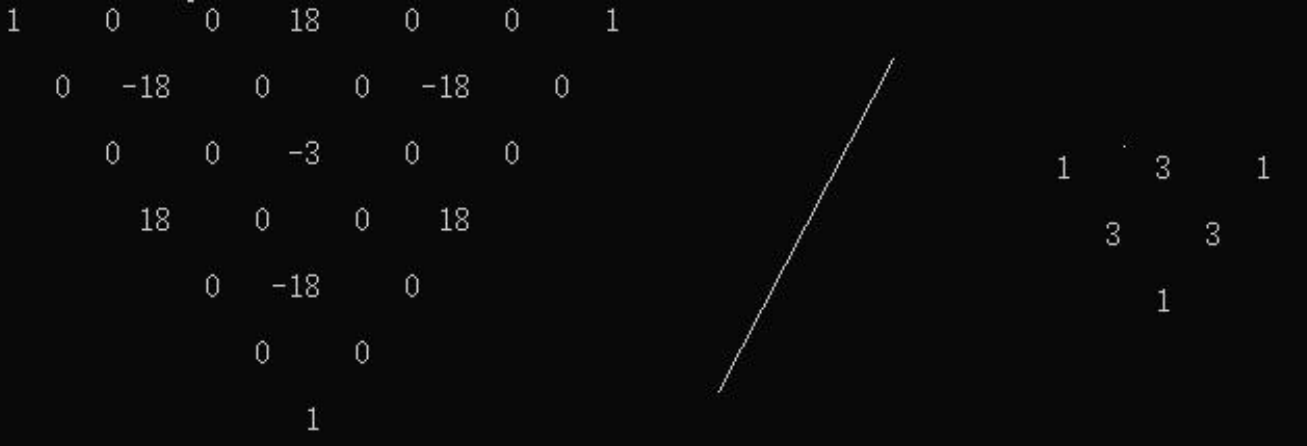
\includegraphics[width=0.8\linewidth]{28}
\end{center}
比如这个(前面考虑到$ [1,3,1]|[1,0,0,18,0,0,1] $所以作这个尝试
\begin{center}
	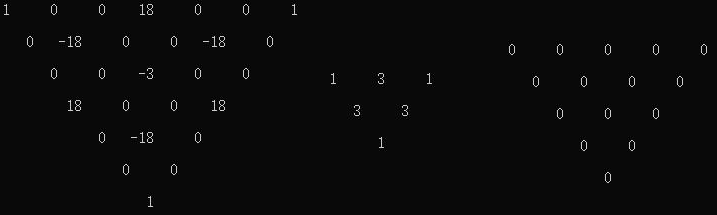
\includegraphics[width=0.5\linewidth]{29}
\end{center}
那么我们先戳个四次的阵当作结果
\begin{center}
	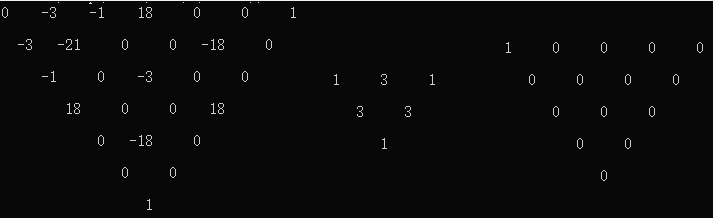
\includegraphics[width=0.8\linewidth]{30}
\end{center}
然后从左上角开始
\begin{center}
	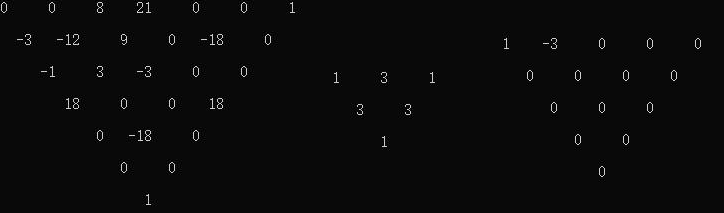
\includegraphics[width=0.8\linewidth]{31}
\end{center}
这样一个个减下来就行了,情况特殊的话可以稍作变化,比如这里知道结果是轮换对称的,就可以一次性拿$ a^4+b^4+c^4 $
\subsection{配方法引入}
那么开始配方法的引入,这要从“想出一个$ (a,b,c)=(1,2,0) $能取等的不等式”开始,想要的还是三元齐次轮换的,那么自然就希望$ F(a,b,0) $和$ (2a-b)^{2} $有点关系。但角上的数得想等,不可能一个$ 1 $一个$ 4 $,最终自然就造出了这个:
\renewcommand*{\arraystretch}{1.732}\[
\left[\begin{matrix}
	0& &4& &-4& &1& &0\\
	&1& &-1& &-1& &4&\\
	& &-4& &-1& &-4& &\\
	& & &4& &1& & &\\
	& & & &0& & & &\\
\end{matrix}\right]
\]
写出来的时候尚且没有确定它是否是非负的。在在没有引入配方法的时候,均值和舒尔自然是难以解决这个问题的,毕竟它应当有$ 111,210,102,021 $四个取等。
\\
那么我们回到代数式来看这个问题是啥,把这些$ [4,-4,1] $理在一起,发现它就是$ \displaystyle \sum ab(2a-b)^{2}\geq abc(a+b+c) $,不禁让人想除掉$ abc $,就是$ \displaystyle \sum \dfrac{(2a-b)^{2}}{c} \geq a+b+c $,到这里我们意识到$ \dfrac{(2a-b)^{2}}{c}+c\geq 2(2a-b) $轮换和一下就行了。\\
现在我们反过来看看$ \dfrac{(2a-b)^{2}}{c}c+c\geq 2(2a-b) $对于系数阵而言有何意味,我们知道基本不等式的一个本质是$ a^{2}+b^{2}\geq 2ab $等价于$ (a-b)^{2}\geq 0 $,所以$ \dfrac{(2a-b)^{2}}{c}+c\geq 2(2a-b) $其实就是$\dfrac{(2a-b-c)^{2}}{c}\geq 0 $,把那个$ abc $乘回来,发现我们做的事就是利用了$ \displaystyle \sum ab(2a-b-c)^{2}\geq 0 $。\\
这时候我们再看看它在系数阵里面对应了什么平方的轮换和:
\renewcommand*{\arraystretch}{1.732}\[
\left[\begin{matrix}
	0& &4& &-4& &1& &0\\
	&0& &-4& &2& &0&\\
	& &0& &1& &0& &\\
	& & &0& &0& & &\\
	& & & &0& & & &\\
\end{matrix}\right]
\]
是这个东西的轮换和,这个平方轮换和一下一定是总和为$ 0 $的,而且边上还一定就是这个$ [4,-4,1] $。于是我们知道了如何以系数阵的视角看这个做法,此后我们就可以直接从系数阵上寻求类似的操作了。\\
例如,\\
$ \left[\begin{matrix}
	0& &9& &-6& &1& &0\\
	&1& &-4& &-4& &9&\\
	& &-6& &-4& &-6& &\\
	& & &9& &1& & &\\
	& & & &0& & & &\\
\end{matrix}\right]
=\displaystyle \sum 
\left[\begin{matrix}
	0& &9& &-6& &1& &0\\
	&0& &-12& &4& &0&\\
	& &0& &4& &0& &\\
	& & &0& &0& & &\\
	& & & &0& & & &\\
\end{matrix}\right] $\\
\begin{3}
	\renewcommand*{\arraystretch}{1.732}\[
	\left[\begin{matrix}
		0& &1& &3& &4& &0\\
		&4& &-2& &-2& &1&\\
		& &3& &-2& &3& &\\
		& & &1& &4& & &\\
		& & & &0& & & &\\
	\end{matrix}\right]
	\]
\end{3}
\begin{4}
	$ [1,-3,4] $不是完全平方,实际上这个东西是松了,但我们依然可以照$ [1,-4,4] $的那个来配,力求把角上的$ 1 $和$ 4 $妥善使用掉,我们拿去三个平方还剩下这个
	\renewcommand*{\arraystretch}{1.732}\[
	\left[\begin{matrix}
		0& &0& &1& &0& &0\\
		&0& &-1& &-1& &0&\\
		& &1& &-1& &1& &\\
		& & &0& &0& & &\\
		& & & &0& & & &\\
	\end{matrix}\right]
	\]
	自然可以基本不等式搞掉
\end{4}
再来一个稍微难一点的
\renewcommand*{\arraystretch}{1.732}\[
\left[\begin{matrix}
	0& &13& &-33& &21& &0\\
	&21& &0& &0& &13&\\
	& &-33& &0& &-33& &\\
	& & &13& &21& & &\\
	& & & &0& & & &\\
\end{matrix}\right]
\]
注:$ 4\times 13\times 21-33^{2}=3 $也即$ 4\times 13\times 21>33^{2} $\\
配方,即$ \displaystyle \sum ab(\sqrt{13}a-\sqrt{21}b+(\sqrt{21}-\sqrt{13})c)^{2}+(\sqrt{13\times 21}-\dfrac{33}{2})\displaystyle \sum c^{2}(a-b)^{2} \geq 0$
我们在配方时往往同时带着“把角上正项消去”和“不放过头”两个意图来拆取平方,这点对于配方法非常重要,如\\
\renewcommand*{\arraystretch}{1.732}\[
\left[\begin{matrix}
	0& &10& &-26& &17& &0\\
	&17& &-1& &-1& &10&\\
	& &-26& &-1& &-26& &\\
	& & &10& &17& & &\\
	& & & &0& & & &\\
\end{matrix}\right]
\]
可以先减掉
$\displaystyle \sum 
\left[\begin{matrix}
	0& &9& &-24& &16& &0\\
	&0& &6& &-8& &0&\\
	& &0& &1& &0& &\\
	& & &0& &0& & &\\
	& & & &0& & & &\\
\end{matrix}\right]
=\displaystyle \sum ab
\left[\begin{matrix}
	3& &-4 \\
	& 1&\\
\end{matrix}\right]^{2} $
,然后还是均值\\
那么我们可以总结一下这种角上为0且齐四次轮换的不等式的通法
\begin{center}
	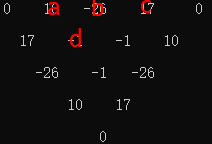
\includegraphics[width=0.3\linewidth]{27}
\end{center}
设这四个位置上的数为$ a,b,c,d $,其中$ a,c> 0 $。首先,考虑到它得以成立,必然要有$ 4ac≥b^{2} $,$ a+b+c+d\geq 0 $。相对地,一旦保证了这四点,就可以拆下一个\\
$ \displaystyle \sum xy(\sqrt{a}x-\sqrt{c}y-(\sqrt{a}-\sqrt{c})z)^{2} $,然后均值即可,此即这类不等式的通法。
那么下面难度升级一下,角上不为零的齐四次轮换对称
\renewcommand*{\arraystretch}{1.732}\[
\left[\begin{matrix}
	1& &-2& &3& &-2& &1\\
	&-2& &0& &0& &-2&\\
	& &3& &0& &3& &\\
	& & &-2& &-2& & &\\
	& & & &1& & & &\\
\end{matrix}\right]
\]
这是$ \dfrac{1}{2}(a-b)^{4} $,但也可以直接考虑$ (\displaystyle \sum (a^{2}-ab))^{2} $
\begin{3}
	$ \dfrac{(\displaystyle \sum a)^{5}}{27} \geq (\displaystyle \sum ab^{2})(\displaystyle \sum ab)$
\end{3}
\begin{4}
	\begin{center}
		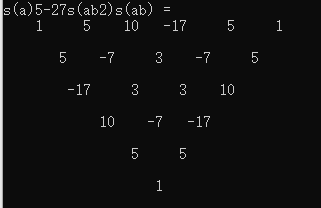
\includegraphics[width=0.5\linewidth]{34}
	\end{center}
	\begin{center}
		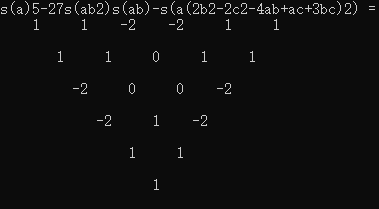
\includegraphics[width=0.5\linewidth]{35}
	\end{center}
	前情提示:Vasc不等式,下面这两题与之类似\\
	已知$ \displaystyle \sum a=2 $,求证:$\displaystyle \sum  \dfrac{a}{1+b^{2}}\geq \dfrac{18}{13} $\\
	已知$ \displaystyle \sum a=3 $,求证:$ 9\geq (\displaystyle \sum a^{2}b)(\displaystyle \sum ab) $
\end{4}
\section{二次元}
\subsection{针对取等的定向配方}
在遇到一些可能不太妙的题目时,除了检查$ f(1,1,1) $这个最平凡的点之外也要注意$ f(a,b,0) $和$ f(a,b,b) $两个特殊的降维情况
看$ f(a,b,b) $时,可以一行一行看总和,然后从下往上念,比如$ [1, -6, 13, -12, 4] $,也就是$ a^{4}-6a^{3}b+13a^{2}b^{2}-12ab^{3}+4b^{4} $,而原不等式有$ a=b=c $取等的话$ f(a,b,b) $必有$ (a-b)^{2} $因式,那么不难发现它其实是$ (a-b)^{2}(a-2b)^{2} $,由此我们会发现原不等式有取等$ (2,1,1) $,
接下来给一个经典的例子
\renewcommand*{\arraystretch}{1.732}\[
\left[\begin{matrix}
	1& &-3& &8& &-3& &1\\
	&-3& &-3& &-3& &-3&\\
	& &8& &-3& &8& &\\
	& & &-3& &-3& & &\\
	& & & &1& & & &\\
\end{matrix}\right]
\]
我们知道既然有取等$ 111,211,121,112 $,那该怎么配方呢?如果我们要拆一个平方,使得减去这个平方后依然非负,那么这个平方肯定在$ 111,211,121,112 $这四个点上取值是$ 0 $,即要覆盖四个取等,类似于两点确定一条直线,我们可以确定一个一次式$ \Box a+\Box b+\Box c $,使得它在$ 111,211 $上都取$ 0 $,即$ b-c $,也可以确定一个在$ 121,112 $上都取$ 0 $的,即$ 3a-b-c $,但实际上我们可以直接利用叉乘得到它,因为这个东西在$ (a,b,c)=(1,2,1) $或$ (1,1,2) $的时候肯定取$ 0 $:
\begin{center}
	$ \begin{vmatrix}
		a& b & c\\
		1& 2 & 1\\
		1& 1 & 2
	\end{vmatrix} $
\end{center}
不会叉乘的话也可以待定系数解线性方程组,那么考虑到$ a^{4} $系数,我们要拆的就是$\dfrac{1}{2} \displaystyle \sum (a-b)^{2}(a+b-3c)^{2} $,拆完之后什么也不剩了,我们姑且把这个技术叫做“针对取等的定向配方”。\\
\begin{3}
	求一个关于$ a,b,c $的齐一次式使得$ (a,b,c)=(1,2,3),(2,3,1) $时都取到零
\end{3}
\begin{4}
	......
\end{4}
\begin{1}
	求证:$ 4(x+y+z)^{3}\ge 27(x^{2}y+y^{2}z+z^{2}x+xyz) $
\end{1}
\begin{2}
	即证
	$ \left[\begin{matrix}
		4& &-15& &12& &4\\
		&12& &-3& &-15&\\
		& &-15& &12& & \\
		& & &4& & &\\
	\end{matrix}\right] \ge 0$\\
	注意到$ 210 $是它的取等,但定向配方配出来会是四次的,所以可以给它乘上$ a+b+c $再拆定向配方\\
	问题:我怎么知道要乘上去的因子是什么?\\
	我们要保证拆的东西对上取等,但上次的方法只能得到四次的,所以至少升一次,那么为了对称就用$ a+b+c $了,升次一般会增大可操作性,但升的太高会难算,要权衡。\\
	怎么注意到取等条件的?\\
	这里是检查$ f(a,b,0) $\\
	最后就是$ \displaystyle \sum (2a-b-c)^{2}(a-2b+4c)^{2}$
	
	注意到$ [1,-4,4]|[4,-15,12,4] $
	\begin{center}
		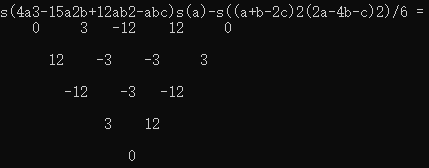
\includegraphics[width=0.5\linewidth]{32}
	\end{center}
	拆完之后是这个,正好和配方最开始的那个例题很像,毕竟拆剩下来的东西肯定也是有那四个取等,所以也只能是这个东西的若干倍了。\\
	其实还有个不乘$ a+b+c $的做法:我们考虑把第一行减完,第一行即$ [1,-4,4]·[4,1] $,所以我们拆个$ (a-2b+c)^{2}(4a+b) $得到$ \left[\begin{matrix}
		0& &0& &0& &0\\
		&4& &11& &-11&\\
		& &-19& &11& & \\
		& & &4& & &\\
	\end{matrix}\right] $
    应该能看出来这是$ c(4(a-c)^{2}+11(a-b)(b-c)) $,毕竟那三个11很显眼,所以设个b为中位数就能保证它非负了
    \begin{center}
    	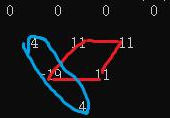
\includegraphics[width=0.3\linewidth]{33}
    \end{center}
    那么这里有个隐藏知识点:“不妨$ b $为中位数”之下,$ (a-b)(b-c) $就是一个非负原件了,那么有些小朋友可能会补充说$ (a-b)(a-c) $、$ (a-c)(b-c) $也是非负的,但其实后两个不用单独拎出来说,因为它们可以认为是$ (a-b)(b-c $)的延伸,其中$ (a-b)(a-c)=(a-b)(b-c)+(a-b)^{2} $,$ (a-c)(b-c)=(a-b)(b-c)+(b-c)^{2} $,所以究其本源的话注意$ (a-b)(b-c) $是非负元件就行了
\end{2}
\subsection{二次元}
我们先给出一个使得(a,b,c)=(1,1,1),(1,2,3),(2,3,1),(3,1,2)都能取等的恒大于零的齐四次轮换不等式:$ \displaystyle \sum (a-2b+c)^{2}(5a-b-7c)^{2} $
再计算这个被平方式本身的轮换和$ \displaystyle \sum (a-2b+c)(5a-b-7c) $,发现居然是$ 0 $\\
实际上我们不难证明,如果一个齐二次式在$ (1,1,1)(p,q,r)(q,r,p)(r,p,q) $处都取$ 0 $,且其中$ p,q,r $不全相等,那么它的轮换和必为$ 0 $,我们把这样的二次式称作二次元。这个点对于齐四次中有特殊取等的不等式(如vasile不等式)很重要,我们把这样的二次式称作二次元,例如$ (a^{2}+b^{2}+c^{2})^{2}\geq 3a^{3}b+3b^{3}c+3c^{3}a $
\begin{1}
设$ x_{a} $是一个二次元(它轮换后的为$ x_{b} $、$ x_{c} $),求$ \dfrac{\displaystyle \sum (x_{a}+x_{b})^{2}}{\displaystyle \sum (x_{a})^{2}}$,注意二次元必有$ \displaystyle \sum x_{a}=0 $	
\end{1}
\begin{2}
	......
\end{2}
\begin{1}
	\renewcommand*{\arraystretch}{1.732}\[
	\left[\begin{matrix}
		1& &1& &0& &-2& &1\\
		&-2& &0& &0& &1&\\
		& &0& &0& &0& &\\
		& & &1& &-2& & &\\
		& & & &1& & & &\\
	\end{matrix}\right]
	\]
\end{1}
\begin{2}
	$ \dfrac{1}{2}\sum (a^{2}-b^{2}-(ac-ab))^{2} $
\end{2}
\begin{1}
	求$ \left[\begin{matrix}
		1& &-2& &2\\
		&-1& &3&\\
		& &-3& &\\
	\end{matrix}\right] $
的平方,然后对结果求轮换和,并解释为什么结果有$ 14 $这么个挺大的因数
\end{1}
\begin{2}
	其平方为$ \left[\begin{matrix}
		1& &-4& &8& &-8& &4\\
		&-2& &10& &-16& &12&\\
		& &-5& &6& &-3& &\\
		& & &6& &-18& & &\\
		& & & &9& & & &\\
	\end{matrix}\right] $,\\
   其轮换和为$ \left[\begin{matrix}
   	14& &14& &0& &-28& &14\\
   	&-28& &0& &0& &14&\\
   	& &0& &0& &0& &\\
   	& & &14& &-28& & &\\
   	& & & &14& & & &\\
   \end{matrix}\right] $
会发现它有挺大的公因数$ 14 $,之后讲到vasile的时候会说这个的。\\
提示:这个被平方的东西轮换和为$ 0 $,设那个是$ x_a $,那么$ \displaystyle \sum x_a^{2} $理应和$ \displaystyle \sum(x_a-2x_b)^{2} $有线性关系,$ x_a-2x_b $是$ \left[\begin{matrix}
	7& &0& &0\\
	&-7& &7&\\
	& &-7& &\\
\end{matrix}\right] $,也就是说$ \displaystyle \sum x_a^{2} $应该是$ \displaystyle \sum (a^{2}-c^{2}-ac+bc)^{2} $的若干倍,考虑到它角上的系数是$ 1^{2}+2^{2}+3^{2} $,所以所有的系数都是$ 14 $的倍数就很正常了。\\
这揭示了我们设二次元的时候可以优先考虑$ a^{2}-b^{2}+\Box ab+\Box ac+\Box bc $型的,即不妨$ c^{2} $前的系数是$ 0 $,那么其实vasile如何配方已经差不多出来了,这里就出现了一个神奇的现象,正因为我们知道vasile不等式很强,有个厉害的非平凡取等,所以我们可以轻松地击破它。你已经知道vasile有非平凡的取等了,你尝试考虑它就是$ \dfrac{1}{2} \displaystyle \sum (a^{2}-b^{2}-pac+qbc+(p-q)ab)^{2} $
然后根据$ a^{3}b $和$ ab^{3} $系数解一下$ p,q $试试,然后确认一下$ a^{2}b^{2} $系数即可,实际上就是$ p=1 $,$ q=2 $(第三个可以设为$ p-q $的原因是其轮换和是$ 0 $)
\end{2}

\subsection{vasile不等式}
\begin{center}
	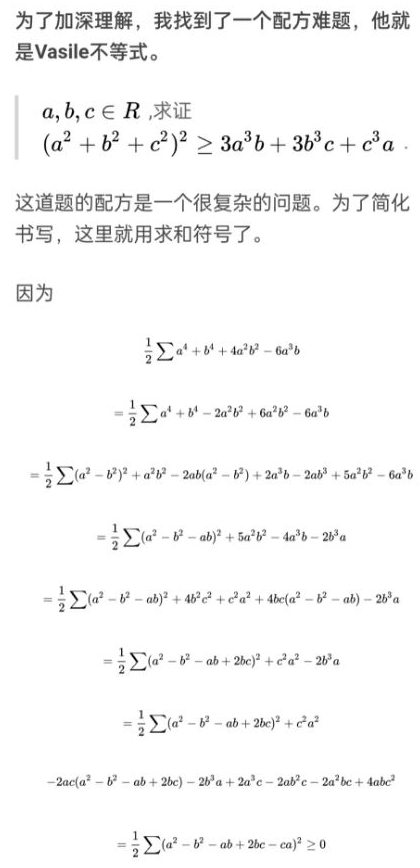
\includegraphics[width=0.6\linewidth]{352}
\end{center}
\begin{1}
	$ \dfrac{(a+b+c)(a^{3}+b^{3}+c^{3})}{3 a b c}\ge \dfrac{a^{2}}{b}+\dfrac{b^{2}}{c}+\dfrac{c^{2}}{a}  $
\end{1}
\begin{2}
	证明:最后配出来的结果是$ \dfrac{1}{2}\sum (a^{2}-b^{2}-(ac-ab))^{2} $
\end{2}
(苏州\quad 褚小光)
\begin{center}
	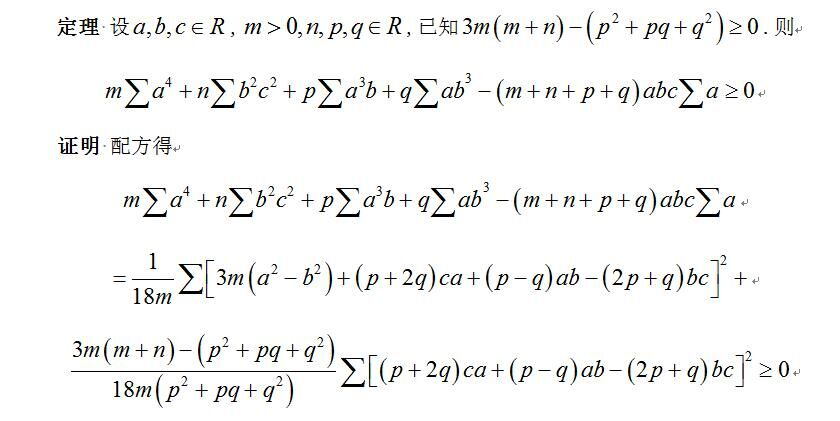
\includegraphics[width=0.8\linewidth]{b01}
\end{center}
\begin{center}
	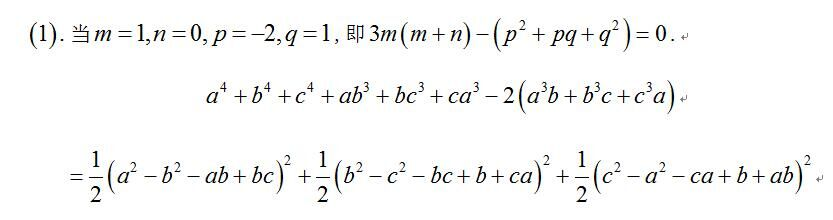
\includegraphics[width=0.8\linewidth]{b02}
\end{center}
\begin{center}
	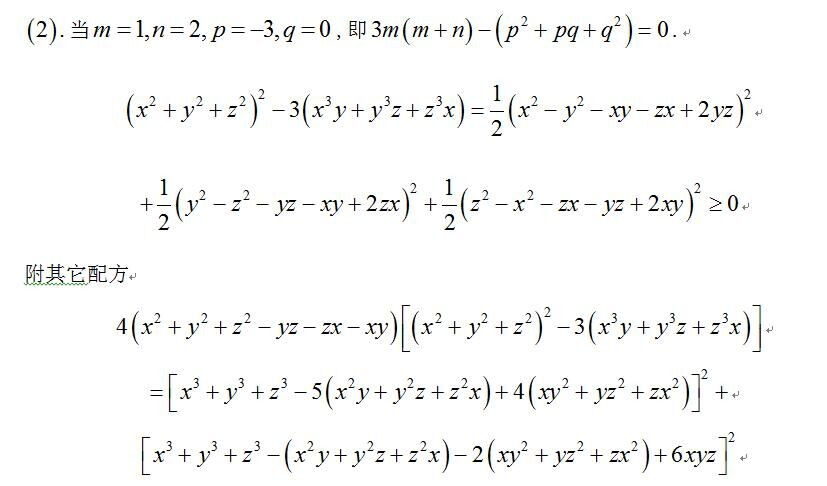
\includegraphics[width=0.8\linewidth]{b03}
\end{center}
\section{sos}
\subsection{一般方法}
sos(sum of squares)
简单来说,它给出了几个根据$ S_{a} $、$ S_{b} $、$ S_{c} $来判定$ \displaystyle \sum S_{a}·(b-c)^{2} $非负性的条件,称其sos定理,于是可以通过配成$ \displaystyle \sum S_{a}·(b-c)^{2} $并验证sos条件的方式来给出证明。\\
在系数阵中,从外往里拆$ [1,-2,1] $就行
\begin{center}
	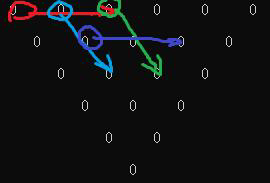
\includegraphics[width=0.4\linewidth]{37}
\end{center}
\begin{center}
	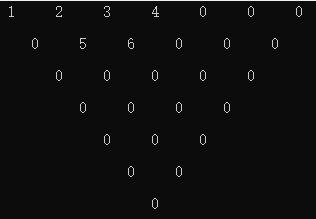
\includegraphics[width=0.4\linewidth]{45}
\end{center}
一般是按照这个顺序,$ 6 $这个拆完剩的肯定是$ 0 $了($ a=b=c $能取等的话)
\subsection{例题}
比如这个,姑且只管配出sos,不管配出来符不符合sos定理的判定
\begin{center}
	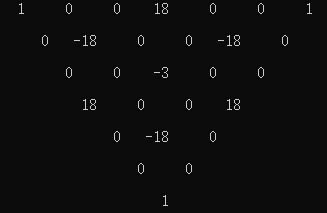
\includegraphics[width=0.5\linewidth]{38}
\end{center}
最外面的是1,考虑把它弄掉
\begin{center}
	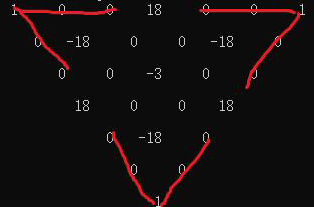
\includegraphics[width=0.5\linewidth]{39}
\end{center}
那么为保对称性可以拆这几个,也就是$ \displaystyle \sum (a^4+b^4)(a-b)^2 $,为了把$ 1 $拆掉所以取$ \dfrac{1}{2} $倍
\begin{center}
	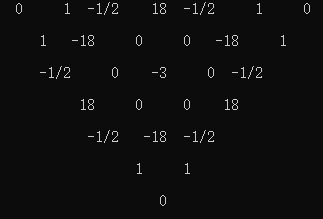
\includegraphics[width=0.5\linewidth]{40}
\end{center}
拆下来就剩这些了,下一个是那些1
\begin{center}
	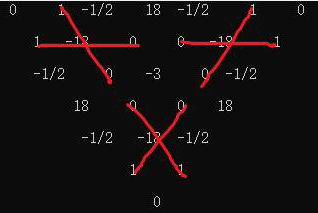
\includegraphics[width=0.5\linewidth]{41}
\end{center}
那么拆这些,也就是$ 1\displaystyle \sum (a^3c+b^3c)(a-b)^2 $
\begin{center}
	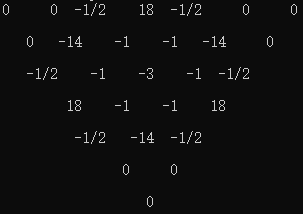
\includegraphics[width=0.5\linewidth]{42}
\end{center}
拆完剩这些,再搞这个-1/2
\begin{center}
	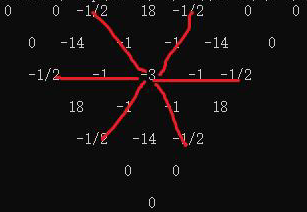
\includegraphics[width=0.5\linewidth]{43}
\end{center}
还是往里伸,那么按红蓝绿紫这个顺序拆到最后就行了
\begin{center}
	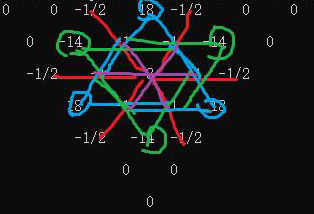
\includegraphics[width=0.5\linewidth]{44}
\end{center}
\pageref{1}\label{2}前面我们留下了这个问题,现在可以解决了:
\begin{center}
	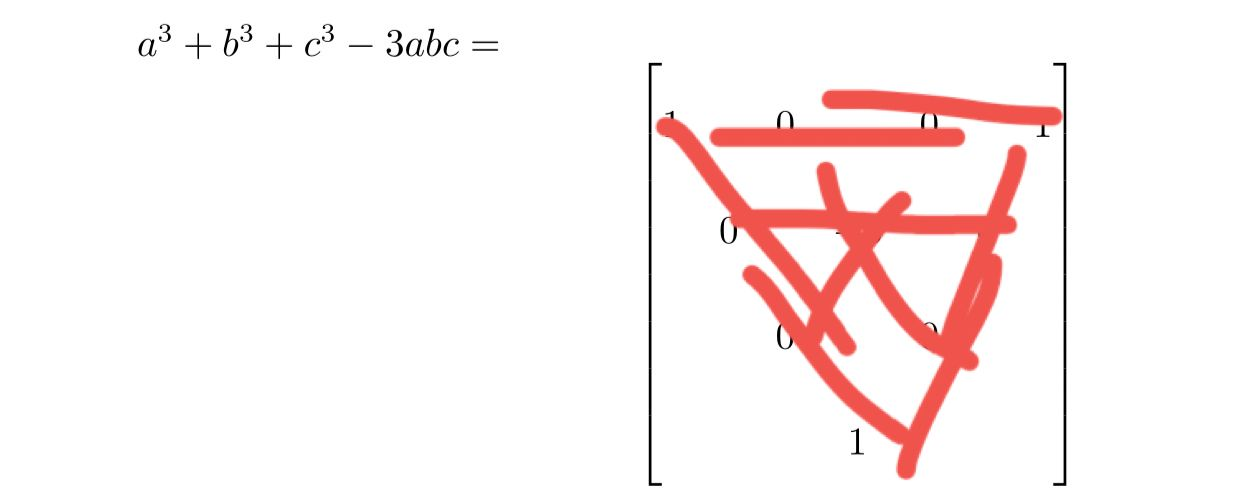
\includegraphics[width=0.7\linewidth]{441}
\end{center}
方便看,先乘2:
\begin{center}
	\includegraphics[width=0.3\linewidth]{442}
\end{center}
然后
\begin{center}
	\includegraphics[width=0.5\linewidth]{443}
\end{center}
结束了\\
也就是:注意到$ 2(a^{3}+b^{3}+b^{3}-3 abc)= \displaystyle \sum _{sym}a(a-b)^{2}+\displaystyle \sum c(a-b)^{2}\ge 0$故得证.
\subsection{习题}
如果不是全相等取等(比如Jack Garfunkel),用系数阵也由外向内也能类似地配出$ \displaystyle \sum S_a (a-3b)^{2} $\\
用待定系数Cauchy处理Garfunkel不等式之后剩下的就是这个:\\
$ 5\displaystyle \prod (a+b)(5a+b+9c)-16\displaystyle \sum a\displaystyle \sum a(b+c)(c+a)(5b+c+9a)(5c+a+9b)\geq 0 $留做习题\\
答案:
$ \sum ab(a+b)(a+9b)(a-3b)^2 +243\sum a^3b^2c + 835\sum a^3bc^3 +232\sum a^4bc + 1230\sum a^2b^2c^2 \ge 0 $
\section{习题}
\noindent$ (1)\displaystyle \sum a^{2}(a-b)(4b+c)\geq 0\\
(2)\displaystyle \sum a^{4}+8\displaystyle \sum a^{2}b^{2}\geq 3\displaystyle \sum a^{2}\displaystyle \sum ab\\
(3)\displaystyle \sum \dfrac{(a^{2}+bc)^{2}}{ab}\geq 4\displaystyle \sum a^{2}\\
(4)4(\displaystyle \sum a)^{3}\geq 27(\displaystyle \sum a^{2}b+abc)\\
(5)\displaystyle \sum \dfrac{a}{b}\displaystyle \sum \dfrac{a}{c}+18\geq 3\displaystyle \sum a\displaystyle \sum \dfrac{1}{a}\\
(6)\displaystyle \sum (a-b)(a^{4}-2b^{3}c+3b^{2}c^{2})\geq 0\\
(7)\displaystyle \sum \dfrac{a^{2}}{(b-c)^{2}} \geq 2\\
(8)\displaystyle \sum \dfrac{(a-b-c)^{4}}{bc}\geq \displaystyle \sum (3a-b-c)^{2}\\
(9)\displaystyle \sum \dfrac{a^{2}}{(a+b)^{2}+(a+c)^{2}}\geq \dfrac{3}{8}\\
(10)\displaystyle \sum \dfrac{a}{b}(4a-3b-c)^{2}\geq 10\displaystyle \sum (a-b)^{2} $
\section{其他}
\subsection{非齐次多项式}
简单的倒是可以按次数分层,然后靠$ (a-1)^{2} $这种东西达到次数之间的相互照应,各层如果都非负的话当然就证完了,但情况肯定没这么好,所以可以用上下层来补到中间,比方说$ (a-1)^{2} $就是拿高层和低层的各一个1补到中间层,当然这样虽然简单但效益低,后面其实就是在说“每层都可以直接用简单的SOS显式完成”
\begin{1}
	韦东奕不等式:设$ a,b,c> 0 $,证明:\\
	\begin{center}
		$ \displaystyle \sum (1-a)^{2}\geq \displaystyle \sum \dfrac{a^{2}(1-b)^{2}(1-c)^{2}}{(a+bc)^{2}} $
	\end{center}
\end{1}
\begin{2}
	\href{https://mp.weixin.qq.com/s/HswqcHJEWK8s-WV68PIqog}{公众号}
	\begin{center}
		\includegraphics[width=0.8\linewidth]{46}
	\end{center}
\end{2}
\subsection{去根号}
这里介绍如何去掉“三个根式的和”一类根号。要
证$ \sqrt{A}+\sqrt{B}+\sqrt{C}\ge \sqrt{D} $先讨论,倘若左边有两个之和已经不小于右边,则得证。否则我们只需考虑$ \prod (i\sqrt{A}+j\sqrt{B}+k\sqrt{C}+\sqrt{D}) $的正负性,对$ i,j,k\in \left \{ 1,-1 \right \}  $求积(乘的7个都是正的),这个式子自然就没有根号了,但是次数会变为原来八倍,所以并不实用。
\section{一些问题}
和系数阵有关或无关的,有答案或没答案的零散问题,暂时还没有归类。
\subsection{}
求证:$ \displaystyle \dfrac{x^{3}+y^{3}+z^{3}}{3 x y z}+\displaystyle \dfrac{3 \sqrt[3]{x y z}}{x+y+z} \geq 2(x, y, z>0) $
证明:
$$ (x, y, z)=(a^{3}, b^{3}, c^{3}) $$
$$3 x y z(x+y+z)(\displaystyle \dfrac{x^{3}+y^{3}+z^{3}}{3 x y z}+\displaystyle \dfrac{3 \sqrt[3]{x y z}}{x+y+z}-2) $$
$$ =\displaystyle \sum a^{4}(a^{4}-b^{4})(a^{4}-c^{4})+\displaystyle \sum c^{8}(a^{2}-b^{2})^{2}+\displaystyle \sum c^{3}(a^{3}+b^{3})(a^{3}-b^{3})^{2} $$
$$ +2 a^{2} b^{2} c^{2}(\displaystyle \sum a^{2}(a^{2}-b^{2})(a^{2}-c^{2})+\displaystyle \sum c^{4}(a-b)^{2}) $$
\subsection{}
\begin{center}
	\includegraphics[width=0.6\linewidth]{a01}
\end{center}
\begin{center}
	\includegraphics[width=0.7\linewidth]{a02}
\end{center}
通分后的系数是这样
\begin{center}
	\includegraphics[width=0.7\linewidth]{a03}
\end{center}
注意到$ ab $边上总和为0,所以先schur一下,再在三条边上各自配,中间-27随便搞,我这个配的不是很好看…仔细一看其实上来拿$  \displaystyle \sum a^{6}(a-b)(a-c) $更舒服。其实这里有个小知识点,由于abc=110取等,所以角上这个1要小心用,得保证$ (a,b,c)=(1,1,0) $和$ (1,0,1) $时候都取得到等,为此我们就可以考虑schur了,因为众所周知schur的取等有$ 111,110,101,011 $四个
\begin{center}
	\includegraphics[width=0.7\linewidth]{a04}
\end{center}
那么拿完$  \displaystyle \sum a^{6}(a-b)(a-c) $ 之后是这样,三条边上刚好是$ [3,-6,3][7,-14,7][3,-6,3] $合起来,中间$ -27 $真的就随便搞了
\begin{center}
	\includegraphics[width=0.9\linewidth]{a05}
\end{center}
\subsection{}
\begin{center}
	\includegraphics[width=0.7\linewidth]{a06}
\end{center}
\begin{center}
	\includegraphics[width=0.7\linewidth]{a07}
\end{center}
\begin{center}
	\includegraphics[width=0.7\linewidth]{a08}
\end{center}
\begin{center}
	\includegraphics[width=0.7\linewidth]{a09}
\end{center}
\subsection{}
\renewcommand*{\arraystretch}{1.732}\[
\left[\begin{matrix}
	\begin{tabular}{ccccccccccccc}
		2& &-2& &-1& &2& &-1& &-2& &2\\
		&-2& &4& &-1& &-1& &4& &-2&\\
		& &-1& &-1& &0& &-1& &-1& &\\
		& & &2& &-1& &-1& &2& & &\\
		& & & &-1& &4& &1& & & &\\
		& & & & &-2& &-2& & & & &\\
		& & & & & &2& & & & & &\\
	\end{tabular}
\end{matrix}\right]
\] 
首先注意到111,110都取等
\begin{center}
	\includegraphics[width=0.7\linewidth]{a10}
\end{center}
考虑到这是六次的,而且角上是$ 1 $,次角负的不多,所以先砸个$ (\displaystyle \sum a(a-b)(a-c))^{2} $下去,这是一个好用的结构
\begin{center}
	\includegraphics[width=0.7\linewidth]{a11}
\end{center}
这里是只减了一份,减两份应该也行,现在我们有余裕用六阶的schur了
\begin{center}
	\includegraphics[width=0.7\linewidth]{a12}
\end{center}
减掉六阶schur之后变这样,可以看出现在难搞的是这个$ -5 $,与此同时必须保证110时的取等,边上这个$ [1,0,-2,0,1] $看上去不太好动,但其实还是有油水可以榨的,因为$ [1,0,-2,0,1]=[0,4,-8,4,0]+[1,-4,6,-4,1] $,所以拿个$ [0,4,-8,4,0] $依然不会死掉,因此这里是可以考虑拿$ 4 $个$ (a-b)^{2}(a-c)^{2}(b-c)^{2} $
\begin{center}
	\includegraphics[width=0.4\linewidth]{a13}
\end{center}
$ (a-b)^{2}(a-c)^{2}(b-c)^{2} $的系数阵,重要。拿$ 4 $个自然是稳的,但实际上拿$ \dfrac{5}{2} $个就够了
\subsection{}
\renewcommand*{\arraystretch}{1.732}\[
\left[\begin{matrix}
	\begin{tabular}{ccccccccccccc}
		0& &1& &2& &1& &0& &0\\
		&0& &-7& &3& &-7& &1&\\
		& &1& &3& &3& &2& &\\
		& & &2& &-7& &1& & &\\
		& & & &1& &0& & & &\\
		& & & & &0& & & & &\\
	\end{tabular}
\end{matrix}\right]
\]
以a4b角位上的1作桩,看能配什么方出来,红点的是桩
\begin{center}
	\includegraphics[width=0.4\linewidth]{a14}
\end{center}
为了消去角,决定让被平方式是这个样子,那么原来2的位置剩下的是$ 2-2·1·(-1)-x^{2} $考虑图省事把这个2也消掉,那么应该$ x=2 $,也就是说我们提的是$ \displaystyle \sum b(a-b)^{2}(a-2c)^{2} $
\begin{center}
	\includegraphics[width=0.5\linewidth]{a15}
\end{center}
减完确实做完了。\\
综上,原不等式等价于$ \displaystyle \sum b(a-b)^{2}(a-2c)^{2}+\dfrac{1}{2}abc\displaystyle \sum (a-b)^{2} \geq 0$
\subsection{}
\begin{center}
	\includegraphics[width=1\linewidth]{a16}
\end{center}
思路和上一题很像
\subsection{}
\begin{center}
	\includegraphics[width=0.8\linewidth]{a17}
\end{center}
\begin{center}
	\includegraphics[width=0.5\linewidth]{a18}
\end{center}
\begin{center}
	\includegraphics[width=0.5\linewidth]{a19}
\end{center}
\subsection{}
已知$ \displaystyle \sum ab=1$,求证$ \displaystyle \sum \dfrac{1}{a+b}\geq \dfrac{5}{2}$\\
条件包含$ 2 $次和$ 0 $次,结论化整之后包含$ 3 $次和$ 2 $次,所以为了齐次化只好把结论平方,也就是证明$
4(\displaystyle \sum ab)(\displaystyle \sum (a+b)(a+c))^{2}-25(a+b)^{2}(a+c)^{2}(b+c)^{2}\ge 0 $
\begin{center}
	\includegraphics[width=0.5\linewidth]{a20}
\end{center}
三条边上各自解决,中间全是正的,松但是$ \dfrac{5}{2} $是最佳系数,因为是$ 110 $趋于取等。
\subsection{}$ a,b,c> 0 $,证明:
$ \dfrac{b}{a+c}+\dfrac{c}{a+b}+\dfrac{9a}{b+c}+\dfrac{16bc}{(b+c)^{2}} \geq 6$
然后会发现$ (a,b,c)~(1,3,0),(1,0,3)(0,1,1) $这三个取等,但$ (1,1,1) $不是取等
$ \left[\begin{matrix}
	0& &9& &3& &-5& &1\\
	&9& &22& &10& &-4&\\
	& &3& &10& &6& &\\
	& & &-5& &-4& & &\\
	& & & &1& & & &\\
\end{matrix}\right] $
与此同时发现$ f(0,b,c) $就是$ (b-c)^4 $,那么一开始要拿的平方就很明白了
$ \left[\begin{matrix}
	0& &-3& &1\\
	&-3& &-2&\\
	& &1& &\\
\end{matrix}\right] $
$ \left[\begin{matrix}
	0& &9& &-6& &1& &0\\
	&9& &4& &4& &0&\\
	& &-6& &4& &0& &\\
	& & &1& &0& & &\\
	& & & &0& & & &\\
\end{matrix}\right] $
拿完剩下这些,自然而然地拆$ (3a-b-c)^{2} $,即
\begin{center}
	\includegraphics[width=1\linewidth]{a21}
\end{center}
其实直接$ ab(3a-b)^{2}+ac(3a-c)^{2}+4abc(a+b+c) $也行
\subsection{}
\begin{center}
	\includegraphics[width=0.8\linewidth]{a22}
\end{center}
\begin{center}
	\includegraphics[width=0.8\linewidth]{a23}
\end{center}
其中$ \sum(a^{2}+\frac{9}{4} b c) \sum(a-b)^{2}(a+b-\frac{9}{4} c)^{2} $是$ abc=1 $条件下的一个重要结构:
\begin{center}
	\includegraphics[width=0.7\linewidth]{a230}
\end{center}
最后代码是
$ s((a3+b3)3)-8p(a)s(a6)-s(a3(a3+b3-3abc+c3)2)-s(a(a2-bc)4)-p(a)s(a2+9/4ab)s((a-b)2(a+b-9/4c)2)-15/8p(a2)(s(a3)-3abc)-55/32abc(s(a3b3)-3p(a2)) $
\subsection{}
\begin{center}
	\includegraphics[width=0.5\linewidth]{a24}
\end{center}
\href{https://artofproblemsolving.com/community/q1h141869p802507}{AoPS}
\subsection{}
\begin{center}
	\includegraphics[width=0.8\linewidth]{a25}
\end{center}
\begin{center}
	\includegraphics[width=0.8\linewidth]{a26}
\end{center}
\href{https://math.stackexchange.com/questions/3527494/}{AoPS}
\begin{center}
	\includegraphics[width=0.7\linewidth]{a27}
\end{center}
\subsection{}
\begin{center}
	\includegraphics[width=1\linewidth]{a28}
\end{center}
其实你可以把它摆正,看起来舒服点(其实是$ (x^{3},y^{3},z^{3})=(a^{2}b,b^{2}c,c^{2}a) $这样的变换,会使得整个阵仿射变换,那么前后问题自然是等价的)
\begin{center}
	\includegraphics[width=0.85\linewidth]{a29}
\end{center}
然后用两次基本模型搞定:$ \displaystyle \sum (a9+3a3b3(a3+b3)-5a7bc-4a4b4c+2a3b3c3)-\displaystyle \sum (a3)\displaystyle \sum (a2+2ab)\displaystyle \sum ((a-b)2(a+b-2c)2)/2-abc\displaystyle \sum (a2+7/3ab)\displaystyle \sum ((a-b)2(a+b-7/3c)2)/2 $\\
基本模型指这个$ \displaystyle \sum (a2+\Box ab)\displaystyle \sum ((a-b)2(a+b-\Box c)2)/2 $,其特点如这些例子
\begin{center}
	\includegraphics[width=0.6\linewidth]{a30}
\end{center}
\subsection{}
$ a, b, c>0  $, 求证:
$ \dfrac{3 a^{4}+a^{2} b^{2}}{a^{3}+b^{3}}+\dfrac{3 b^{4}+b^{2} c^{2}}{b^{3}+c^{3}}+\dfrac{3 c^{4}+c^{2} a^{2}}{c^{3}+a^{3}} \geq 2(a+b+c) $ (韩京俊)\\
证明:注意到$ \displaystyle \sum (b^{3}+c^{3})(c^{3}+a^{3})(3 a^{4}+a^{2} b^{2})-2(\displaystyle \sum  a)(\prod a^{3}+b^{3})= \\
\displaystyle \sum  a^{3} b^{3}(a-b)^{4}+\displaystyle \sum  a^{4} b^{2}(a-b)^{2}(b+c)^{2}+ 
\displaystyle \sum  a^{4} b^{2}(2 a b-b^{2}-a c)^{2}+\\
\displaystyle \sum  a b(a^{2} b^{2}-\dfrac{5}{2} a b^{2} c+\dfrac{1}{2} a^{2} b c-a^{2} c^{2}-b^{2} c^{2}+3 a b c^{2})^{2}+ \\
\dfrac{1}{2} a^{2} b^{2} c^{2} \displaystyle \sum (a^{2}-b^{2}-\dfrac{35}{12}(c a-a b)+\dfrac{19}{12}(b c-a b))^{2}+\dfrac{5}{96} a^{2} b^{2} c^{2} \displaystyle \sum (a-b)^{2} c^{2} \geq 0  $故得证.\\
(代码$ s((b3+c3)(c3+a3)(3a4+a2b2))-2s(a)p(a3+b3)-s(ab(a3b-2a2b2+ab3)2)-s(a3b2-a2b3+a3bc-a2b2c)2-s((2a3b2-a2b3-a3bc)2)-s(ab(a2b2-5/2ab2c+1/2a2bc-a2c2-b2c2+3abc2)2)-1/2p(a)2s((a2-b2-35/12(ac-ab)+19/12(bc-ab))2)-5/96p(a)2s(c2(a-b)2) $)
\subsection{}
已知$  a, b, c \geq 0 $ 求证:
$ \dfrac{a b}{c^{2}+a b}+\dfrac{b c}{a^{2}+b c}+\dfrac{c a}{b^{2}+c a} \geq \dfrac{4 a b c}{(a+b)(b+c)(c+a)}+1 $
\begin{center}
	\includegraphics[width=0.5\linewidth]{a31}
\end{center}
可以发现不升次数难以解决,于是我们乘一个$ a+b+c $:
\begin{center}
	\includegraphics[width=0.5\linewidth]{a32}
\end{center}
然后分成这三部分结束,也就是:\\
注意到$ (a+b+c)[\sum ab(a^{2}+bc)(b^{2}+ca)\prod (a+b)-(4abc+\prod (a+b))\prod (c^{2}+ab)]=\\
2\sum a^{3}b^{3}c(a-b)^{2}(a+b)+\sum  a^{2}b^{2}c^{3}(a-b)^{2}(a+b)+\sum a^{2}b^{2}c(a^{2}-b^{2})(a^{3}-b^{3})\ge 0 $故得证!
\subsection{}
 $ a, b, c>0 $ .求证:$ (a b+b c+c a)^{3} \geq(-a+b+c)(a-b+c)(a+b-c)(a+b+c)^{3} $
\begin{center}
	\includegraphics[width=0.5\linewidth]{a33}
\end{center}
显然能得到$ (\sum ab)^3-(a+b+c)^3\prod (-a+b+c)=\\
abc\sum (a-b)(a^2-b^2)+\dfrac{1}{2} \sum (a^2-b^2)(a^4-b^4)+\dfrac{1}{2} \sum ab(a-b)(a^3-b^3)+\dfrac{3}{2}\sum ab(a^2-b^2)^2 \ge 0 $故得证!
\subsection{}
已知:  $ a, b, c \in R^{+} $ , 证明:$ (a+b+c)^{3}(a^{3}+b^{3}+c^{3}+a b c) \geq 36 a b c(a^{3}+b^{3}+c^{3}) $
\begin{center}
	\includegraphics[width=0.5\linewidth]{a34}
\end{center}
显然能得到$\sum a^{3}(\sum a^{3}+abc)-36abc(\sum a^{3})=\\
\sum (a^{4}(a-b)(a-c))+4\sum (ac(a-b)^{4})+4\sum (bc(a-b)^{4})+3\sum (c4(a-b)^{2})+2\sum (b^{2}c^{2}(a-b)(a-c))\ge 0$故得证!
\subsection{}
$ a^4+b^4=2,
ab^2+a^2+a^2b+b^2 \le a^2b^2+a^3+b^3+ab $
\begin{center}
	\includegraphics[width=0.5\linewidth]{a37}
\end{center}

\subsection{}
\begin{center}
	\includegraphics[width=0.5\linewidth]{a35}
\end{center}
\begin{center}
	\includegraphics[width=0.5\linewidth]{a36}
\end{center}
\end{document}
\section{预备知识} 
(下面是常用的东西,可以先复制到另一个tex方便复制)
代码里搜这些星常用的符号可以快速替换:(ps:不复制这个容易被你自己替换掉)
² $ ^{2} $
^{3} $ ^{3} $
⁴ $ ^{4} $
Σ $ \displaystyle \sum $
≥ $ \geq 0$
乘$ \prod $
$ 
> < 
\Leftrightarrow 
\Box 
$
交叉引用(前点后,多次编译)\pageref{key}\label{key}
链接
\href{https://www.baidu.com/}{这是百度的链接}
\href{}{}
系数阵专用
(如果要行内的不复制首尾行再加$ $即可)
2
\renewcommand*{\arraystretch}{1.732}\[
\left[\begin{matrix}
	1& &1 \\
	& 1&\\
\end{matrix}\right]
\]
3
\renewcommand*{\arraystretch}{1.732}\[
\left[\begin{matrix}
	0& &0& &0\\
	&0& &0&\\
	& &0& &\\
\end{matrix}\right]
\]
4
\renewcommand*{\arraystretch}{1.732}\[
\left[\begin{matrix}
	0& &0& &0& &0\\
	&0& &0& &0&\\
	& &0& &0& & \\
	& & &0& & &\\
\end{matrix}\right]
\]
5
\renewcommand*{\arraystretch}{1.732}\[
\left[\begin{matrix}
	0& &0& &0& &0& &0\\
	&0& &0& &0& &0&\\
	& &0& &0& &0& &\\
	& & &0& &0& & &\\
	& & & &0& & & &\\
\end{matrix}\right]
\]
6
\renewcommand*{\arraystretch}{1.732}\[
\left[\begin{matrix}
	\begin{tabular}{ccccccccccccc}
		0& &0& &0& &0& &0& &0\\
		&0& &0& &0& &0& &0&\\
		& &0& &0& &0& &0& &\\
		& & &0& &0& &0& & &\\
		& & & &0& &0& & & &\\
		& & & & &0& & & & &\\
	\end{tabular}
\end{matrix}\right]
\]
7
\renewcommand*{\arraystretch}{1.732}\[
\left[\begin{matrix}
	\begin{tabular}{ccccccccccccc}
		0& &0& &0& &0& &0& &0& &0\\
		&0& &0& &0& &0& &0& &0&\\
		& &0& &0& &0& &0& &0& &\\
		& & &0& &0& &0& &0& & &\\
		& & & &0& &0& &0& & & &\\
		& & & & &0& &0& & & & &\\
		& & & & & &0& & & & & &\\
	\end{tabular}
\end{matrix}\right]
\]
8
\renewcommand*{\arraystretch}{1.732}\[
\left[\begin{matrix}
	\begin{tabular}{ccccccccccccccc}
		0& &0& &0& &0& &0& &0& &0& &0\\
		&0& &0& &0& &0& &0& &0& &0&\\
		& &0& &0& &0& &0& &0& &0& &\\
		& & &0& &0& &0& &0& &0& & &\\
		& & & &0& &0& &0& &0& & & &\\
		& & & & &0& &0& &0& & & & &\\
		& & & & & &0& &0& & & & & &\\
		& & & & & & &0& & & & & & &\\
	\end{tabular}
\end{matrix}\right]
\]